\documentclass[letter, 10pt]{article}
\usepackage[T1]{fontenc}
\usepackage{tgpagella}
\usepackage{graphicx,amsmath,amsfonts,amscd,amssymb,bm,url,color,latexsym}
\usepackage{fullpage}
\usepackage[small,bf]{caption}
%\usepackage{subfig}
\usepackage{subcaption}
\usepackage{bbm}
\usepackage{microtype}
\setlength{\captionmargin}{30pt}
\usepackage{algorithm}
\usepackage{algorithmicx}
\usepackage{algpseudocode} 
\usepackage{verbatim}
\usepackage{framed}
\usepackage{comment}
\usepackage{tikz}
\usepackage{fge}
\usepackage{mathtools}

% pagebreak for long equations
\allowdisplaybreaks  

\usepackage{hyperref}
\hypersetup{
    colorlinks=true,%
    citecolor=blue,%
    filecolor=blue,%
    linkcolor=blue,%
    urlcolor=blue
}
\usepackage[toc, page]{appendix}

\usepackage[capitalize]{cleveref}
%%%%%%%%%%%%%%
\renewcommand\floatpagefraction{.95}
\renewcommand\topfraction{.95}
\renewcommand\bottomfraction{.95}
\renewcommand\textfraction{.05}
\setcounter{totalnumber}{50}
\setcounter{topnumber}{50}
\setcounter{bottomnumber}{50}
%%%%%%%%%%%%%%
%--------------
\newtheorem{theorem}{Theorem}[section]
\newtheorem{lemma}[theorem]{Lemma}
\newtheorem{corollary}[theorem]{Corollary}
\newtheorem{proposition}[theorem]{Proposition}
\newtheorem{definition}[theorem]{Definition}
\newtheorem{conjecture}[theorem]{Conjecture}
\newtheorem{problem}[theorem]{Problem}
\newtheorem{claim}[theorem]{Claim}
\newtheorem{remark}[theorem]{Remark}
\newtheorem{example}[theorem]{Example}



\renewcommand{\mathbf}{\boldsymbol} 


\newcommand{\mb}{\mathbf}
\newcommand{\mc}{\mathcal}
\newcommand{\mf}{\mathfrak}
\newcommand{\md}{\mathds}
\newcommand{\bb}{\mathbb}
\newcommand{\magnitude}[1]{ \left| #1 \right| } 
\newcommand{\set}[1]{\left\{ #1 \right\}}
\newcommand{\condset}[2]{ \left\{ #1 \;\middle|\; #2 \right\} }

\newcommand{\reals}{\bb R}
\newcommand{\proj}{\mathrm{proj}}


\newcommand{\eps}{\varepsilon}
\newcommand{\R}{\reals}
\newcommand{\Cp}{\bb C}
\newcommand{\Z}{\bb Z}
\newcommand{\N}{\bb N}
\newcommand{\Sp}{\bb S}
\newcommand{\Ba}{\bb B}
\newcommand{\indicator}[1]{\mathbbm 1_{#1}}

\newcommand{ \Brac }[1]{\left\lbrace #1 \right\rbrace}
\newcommand{ \brac }[1]{\left[ #1 \right]}
\newcommand{ \paren }[1]{ \left( #1 \right) }

% to declare new operator 
% \DeclareMathOperator{\xxx}{xxx}
\DeclareMathOperator{\dist}{dist}
\DeclareMathOperator{\rank}{rank}
\DeclareMathOperator{\trace}{tr}
\DeclareMathOperator{\supp}{supp}
\DeclareMathOperator{\conv}{conv}
\DeclareMathOperator{\vect}{vec}
\DeclareMathOperator{\diag}{diag}
\DeclareMathOperator{\sign}{sign}
\DeclareMathOperator{\grad}{grad}
\DeclareMathOperator{\Hess}{Hess}
\DeclareMathOperator{\mini}{minimize}
\DeclareMathOperator{\maxi}{maximize}
\DeclareMathOperator{\st}{subject\; to}

%% Other definitions 

\newcommand{\event}{\mc E}

\newcommand{\e}{\mathrm{e}}
\newcommand{\im}{\mathrm{i}}
\newcommand{\rconcave}{r_\fgecap}
\newcommand{\Lconcave}{L_\fgecap}
\newcommand{\rconvex}{r_\fgecup}
\newcommand{\Rconvex}{R_\fgecup}
\newcommand{\Lconvex}{L_\fgecup}

\newcommand{\wh}{\widehat}
\newcommand{\wt}{\widetilde}
\newcommand{\ol}{\overline}

\newcommand{\betaconcave}{\beta_\fgecap}
\newcommand{\betagrad}{\beta_{\mathrm{grad}}}

\newcommand{\norm}[2]{\left\| #1 \right\|_{#2}}
\newcommand{\abs}[1]{\left| #1 \right|}
\newcommand{\innerprod}[2]{\left\langle #1,  #2 \right\rangle}
\newcommand{\prob}[1]{\bb P\left[ #1 \right]}
\newcommand{\expect}[1]{\bb E\left[ #1 \right]}
\newcommand{\function}[2]{#1 \left(#2\right)}
\newcommand{\integral}[4]{\int_{#1}^{#2}\; #3\; #4}

\newcommand{\js}[1]{{\color{blue}{\bf Ju: #1}}}
\newcommand{\qq}[1]{{\color{blue}{\bf Qing: #1}}}
\newcommand{\td}[1]{{\color{magenta}{\bf TODO: #1}}}
\newcommand{\jw}[1]{{\color{blue}{\bf John: #1}}}

\numberwithin{equation}{section}

\def \endprf{\hfill {\vrule height6pt width6pt depth0pt}\medskip}
\newenvironment{proof}{\noindent {\bf Proof} }{\endprf\par}

\newcommand{\qed}{{\unskip\nobreak\hfil\penalty50\hskip2em\vadjust{}
           \nobreak\hfil$\Box$\parfillskip=0pt\finalhyphendemerits=0\par}}

\pagestyle{plain}

\title{Sparse Blind Deconvolution}

\author{Qingyun Sun\\
  \vspace{-.1cm}\\
   \emph{Working notes}
}
\date{  \quad Revised: \today}
\date{\today}

\begin{document}
\maketitle

\vspace{-0.3in}
% \begin{abstract}
% In this note, we set out to recover low-rank probability using nonconvex optimization. 
% \end{abstract}

% \noindent \textbf{Keywords.} 
\section{Introduction}
Blind Deconvolution is the problem of recovering a convolutional kernel $w$ and a signal $x$, both with certain structures, from their convolution $y=w*x$. This is a ubiqutous problem in the signal processing, machine learning, communication, sesmiology, computer vision, microscopy, neural science. 

 
\section{Problem}
\subsection{Mathematical Definition}
Mathematically, we define a time series as a doubly infinite sequence $\tilde x=(\ldots, x_{-1}, x_0, x_1, \ldots)\in l_1( \mathbb{Z})$,  namely $\sum_{i=-\infty}^{\infty}|x_i| < \infty$. 
We define the (two-sided) convolution 
$\tilde y=\tilde w*\tilde x$ by 
$$y_t = \sum_{i=-\infty}^{\infty}w_{t-i}x_i.$$

We define Fourier transform $\mathcal F$ on $l_1( \mathbb{Z})$
as $$ \hat y_s = (\mathcal F y)(s) = \sum_{t =-\infty}^\infty y_t 
    \exp \left( -2\pi i ts \right).$$

For two series $w, x \in l_1( \mathbb{Z})$, by convolution theorem, the Fourier transform of $x*w$ is the point-wise product of $\hat x$ and $\hat w$,
$$ \widehat{x*w} = \hat x \cdot \hat w.$$

When $\tilde w \in l_1( \mathbb{Z})$ is nonzero, we can define the convolutional inverse $\tilde w^{-1}$ of $\tilde w\in l_1( \mathbb{Z})$ by $\tilde w^{-1}*\tilde w = \delta_0$.
 We know $l_1( \mathbb{Z})$ is a Banach algebra where the multiplication is convolution operator $*$, therefore, since $\tilde x,\tilde w\in l_1( \mathbb{Z})$, $\tilde y=\tilde w*\tilde x$ and $\tilde w^{-1}$ are in $l_1( \mathbb{Z})$.
  
In practice, we only observe finite dimensional vector. Given a $n$ dimensional vector $ y\in \mathbb{R}^n$ as observation, we can embed the vector as finite-length series $y^n = (\ldots, 0, y_0, y_1, \ldots, y_{n-1}, 0, \ldots)$. The reason we choose the space $l_1( \mathbb{Z})$ is the following: for a finite length $w$, there is no guarantee that there exists a finite length inverse, we need to consider the problem in the space $l_1( \mathbb{Z})$, which is a Banach algebra where the multiplication is convolution operator $*$, so that every nonzero element has an inverse in this space. 

Informally, we want to find a kernel $b\in \mathbb{R}^k$ as an approximate inverse of the convolutional kernel $w$. We hope that $b*y = b*w*x \approx x$. We can identify $b$ as a series $(\ldots, 0, b_0, b_1, \ldots, b_{k-1}, 0, \ldots)$ in the subspace of $ l_1(\mathbb{Z})$. 

\subsection{Convex optimization problem for deconvolution}
We consider the following problem: given a $n-$dimensional vector $ y\in \mathbb{R}^n$ as observation, we try to find an $k$-dimensional vector $b$ with certain structure, so that $x = b*y^n$ is sparse. We assume that the structure of $b$ is imposed by a convex regularizer $R(b)$.

We want to find $b \in \mathbb{R}^k$ such that 
 \begin{eqnarray*}
\underset{b\in \mathbb{R}^k}{\mbox{minimize}}& \|y*b\|_0+R(b) ,\\
\mbox{subject to}& b \neq 0.
 \end{eqnarray*}

Since the objective $\|y*b\|_0$ is non-convex and hard to optimize, we can replace it with the convex norm $\|y*b\|_1$. 

Without loss of generality, we can replace the condition $b \neq 0$ with a linear constraint 
$b_0 =1$ due to the symmetry of convolution, we will explain this in detail below.

We will find $b \in \mathbb{R}^k$ by solving  the following convex optimization problem:
 \begin{eqnarray*}
\underset{b\in \mathbb{R}^k}{\mbox{minimize}}& \|y*b\|_1 ,\\
\mbox{subject to}& b_0 =1.
 \end{eqnarray*}
 



\subsection{The symmetry in the space of solutions }
The equation $y = w * x$ has scale and shift symmetry:
$y = (cw) *(c^{-1}x)$ for $c\in \mathbb{R}$, and also $y = (T_jw) *(T_{-j}x)$ where $T_j$ is the shift operator: $(T_jw)_t = w_{t+j}$.  Therefore, the inverse $b = w^{-1}$ is only determined up to scale and shift. We need to at least fix the scale to get a non-zero solution. Without loss of generality, we can set $b_0 =1$, so that the solution $b^*$ to the above constrained optimization problem satisfy the following: (one of) the entry with maximum absolute value is shifted to index $0$ and the entry is set as $1$ after rescale and sign flip. 

We define the constraint set of $b$ as $B_{k} = \{b\in l_1( [0, k)) |\  b_0 =1\}$, then this a subspace of  $l_1( \mathbb{Z})$.

Taking into account of the inherent nonuniqueness, we define an equivalent relation on non-zero series, by considering $b$ and $\pm T_j(b) $ to be equivalent. We call this equivalent class $S(b)$ and consider solutions in the same equivalent class essentially same, and we consider a induced norm on the space of equivalent classes:
 \begin{eqnarray*}
d(b^1, b^2) = \min_{b'^2 \in S({b^2}}) \|b^1 - b'^2\|_1
 \end{eqnarray*}
 
 
 

 
\section{ADMM for large scale solution}
Now we consider how to solve the problem at large scale.
We use alternating direction method of multipliers(ADMM) to solve the problem:
 \begin{eqnarray*}
\underset{b}{\mbox{minimize}}& \|x\|_1 + R(b),\\
\mbox{subject to}& x = y*z, \\
& b = z, \\
& b_0 =1.
 \end{eqnarray*}
 where $I_{b_0-1}$ is the indicator function on $b_0 =1.$
 
 The augmented Lagrangian for the convex problem is 
\begin{eqnarray*}
 L(b, x , z, u, v)&=&\|x\|_1 + R(b) +s/2 \| b-z-u\|^2 +
 \rho /2 \| x-y*z-v\|^2,
\end{eqnarray*}
where $ b_0 =1$, and $u, v$ are the scaled dual variables.  

ADMM consists of the iterations
\begin{eqnarray*}
x^{t+1}&=&\mathrm{argmin}_{x} L(b^{t}, x , z^{t}, u^{t}, v^{t})
= \mathrm{argmin}_{x} \|x\|_1+ \rho /2 \| x-y*z^{t}-v^{t}\|^2,\\
b^{t+1}&=&\mathrm{argmin}_{b: b_0=1} L(b, x^{t+1} , z^{t}, u^{t}, v^{t})
=\mathrm{argmin}_{b} R(b) +s/2 \| b-z^{t}-u^{t}\|^2,\\
z^{t+1}&=&\mathrm{argmin}_{z} L(b^{t+1}, x^{t+1}, z , u^{t}, v^{t})
= \mathrm{argmin}_{z} s/2 \| b^{t+1}-z-u^{t}\|^2 +
 \rho /2 \| x^{t+1}-y*z-v^{t}\|^2, \\
u^{t+1}&=& u^t + b^{t+1}-z^{t+1},\\
v^{t+1}&=& v^{t}+ (x^{t+1}-y*z^{t+1}).
 \end{eqnarray*}

One advantage of this approach is that we can leverage the convolution theorem, and compute the $z$-update using Fourier transform.  
 \begin{eqnarray*}
 s/2 \| b-z-u\|^2 +
 \rho /2 \| x-y*z-v\|^2 
 = s/2 \| \hat b-\hat z- \hat u\|^2 +
 \rho /2 \| \hat x-\hat y\cdot \hat z-\hat v\|^2,
  \end{eqnarray*}
 Hence  
  \begin{eqnarray*}
 \hat z^{t+1} 
 =\mathrm{argmin}_{\hat z} s/2 \| \hat b-\hat z- \hat u\|^2 +
 \rho /2 \| \hat x-\hat y\cdot \hat z-\hat v\|^2 .
  \end{eqnarray*} 
  This update can be computed on each coordinate
    \begin{eqnarray*}
 \hat z^{t+1}_i
 = (s(\hat b_i- \hat u_i)+\rho \hat y_i (\hat x_i-\hat v_i))/(s +\rho \hat y_i^2)
  \end{eqnarray*} 
 Using Fast Fourier transform, we can compute this update in $O(n\log n)$. 
  
For $x$ update, we just compute soft-thresholding. Similarly, on $b$ update, we just compute the prox operator of $\|\cdot\|_1$:
   \begin{eqnarray*}
 x^{t+1}
 = S_{1/\rho}(y*z^{t}+v^{t}),
  \end{eqnarray*}
  where $S_{1/\rho} (y*z^{t}+v^{t}) = 
  (y*z^{t}+v^{t}-1/\rho)_{+} - (-y*z^{t}-v^{t}-1/\rho)_{+}$.
  
  And for $b$ update, let the proximal operator of $ R(b)$ be $\mbox{prox}_{R, s}(b)$, let $\Pi_{b_0=1}(b)$ be the projection operator on $b_0 =1$, then
     \begin{eqnarray*}
 b^{t+1}
 = \Pi_{b_0=1}(\mbox{prox}_{R, s}(z^t+u^t)).
  \end{eqnarray*}

When $R(b)$ is the indicator function of a convex constraint set, then the proximal operator is the projection onto this constraint set.
  
From the general theory of ADMM, we know that the update will converge to the global minimum. This method takes advantage of the convolution theorem and fast Fourier transform, and it is suited for large scale problem.



%  Using Fourier transform, we can further write it as:
%   \begin{eqnarray*}
% \underset{b}{\mbox{minimize}}& \|x\|_1 + R(b),\\
% \mbox{subject to}& x' = \hat{y} \cdot b', \\
% & x' = \hat{x}, \\
% & b' = \hat{b}, \\
% & b_0 =1.
%  \end{eqnarray*}
 
% The augmented Lagrangian for the convex problem is 
% \begin{eqnarray*}
%  L_{\rho}(b, b', x, x', s, u, v)&=&\|x\|_1 + R(b) +I_{b_0-1} + \rho_1 /2 \| x' - \hat{y} \cdot b'-s\|^2+\rho_2 /2 \| x' - \hat{x} - u\|^2 +\rho_3 /2 \| b' - \hat{b} - v\|^2
% \end{eqnarray*}
% where $I_{b_0-1}$ is the indicator function on $b_0 =1.$
% and $v$ is the scaled dual variable.  

% ADMM consists of the iterations
% \begin{eqnarray*}
% x^{t+1}&=&\mathrm{argmin}_{x} L_{\rho}(\hat{A}, J^{t},U^{t}),\\
% U^{t+1}&=&\mathrm{argmin}_{U} L_{\rho}(\hat{A}^{t+1}, J^{t},U),\\
% J^{t+1}&=&J^{t}+ (\hat{A}^{t+1}-U^{t+1}A).
%  \end{eqnarray*}
 
% From the general theory of ADMM, we know that the update will converge to the global minimum. 
 
 
\section{Theoretical Results}
\subsection{Probabilisitc model}
To state the theoretical result for the simple model:
Assume that we observe sampled data $y\in \mathbb{R}^n$ from doubly infinite series $\tilde y=\tilde w*\tilde x$ in $l_1( \mathbb{Z})$,$x$ is I.I.D. series sampled from a random variable $X$ with probability $1-p$ to be zero, and probability $p$ to be sampled from a sub-Gaussian random variable. 
And for the kernel $w\in l_1( \mathbb{Z})$, we assume that there exist a length $k$ inverse $b^* = w^{-1}$, and $b^*$ has a single entry with maximum absolute value. And we only know the length of $b^*$  $k < n$ no structure of $b^* \in \mathbb{R}^k$, hence we use no regularizer $R(b)$. 

Without loss of generality, since we know there is a single entry of $b^*$ with maximum absolute value, we can assume $b^*_0 =1$. Let the second largest absolute value of $b^*$ be $M_b$.

Then we prove that under certain condition, we can find $b^*$ by solving a convex optimization problem.
 
\begin{theorem}
Under the above assumption, there exists $p^0, k^0, M_b^0$, if $1/n <p< p_0$, $1<k< k^0$, $M_b\leq M_b^0$,
the global optimizer of the following convex optimization problem is $b^*$.
 \begin{eqnarray*}
\underset{b\in\mathbb{R}^k}{\mbox{minimize}}& \|y^n*b\|_1 ,\\
\mbox{subject to}& b_0 =1.
 \end{eqnarray*}
\end{theorem}
\begin{proof}
Let  $I=\{t: (b^**y)_t =0 \}$, $I_+=\{t: (b^**y)_t >0 \}$ and $I_-=\{t: (b^**y)_t <0 \}$. 
Since the problem is convex, to prove that $b^*$ is the global minimizer, we only need to look at the sub-gradient at $b^*$, 
\begin{eqnarray*}
\partial_b\|y*(b)\|_1 |_{b=b^*}.
\end{eqnarray*}
Equivalently, we need to prove that there exists a $\epsilon>0$, for any $d$ such that $\|d\|_1\leq \epsilon, d_0 =0.$   
\begin{eqnarray*}
\|y*(b^*+d)\|_1-\|y*(b^*)\|_1 
&=& \sum_{t\in I} (|(y*d)_t|) + \sum_{t\in I_0^c} (|(y*(b^*+d)_t|- |(y*(b^*)_t|) \\
&= & \sum_{t\in I} (|(y*d)_t|) +\sum_{t\in I_0^c} (\mbox{sgn}((y*b^*)_t)(y*d)_t\\
&= & \sum_{t\in I} (|(y*d)_t|) +\sum_{t\in I_+} (y*d)_t  - \sum_{t\in I_-} (y*d)_t
\end{eqnarray*}
All entries of first term $\sum_{t\in I} (|(y*d)_t|)$ are positive.

Now consider a change of variable:
Since we have $y= w*x$, where $w*b^*=\delta$, we define $f = w*b$ as a change of variable from $b$ to $f$. 
Then the constraint $b_0= \delta_0^T b = 1$ is transformed to $\delta_0^T b^* *f = \delta_0^T C(b^*)f = b^{*,T} f = 1$, then the constraint $ b^{*,T} f = 1$ gives $ f_0 = 1 - \sum_{i\neq 0} b^*_i f_i $. 
Let $f = f'+ f_0 \delta_0$, we can consider the sub-gradient around $f = \delta_0$,
\begin{eqnarray*}
\partial_f\|x*f\|_1 |_{f'=\delta_0}  = \partial_{f'}\|x*(f'+ (1 - \sum_{i\neq 0} b^*_i f_i) \delta_0)\|_1 |_{f'=0}.
\end{eqnarray*}

\begin{eqnarray*}
\|x*f\|_1-\|x*(\delta_0)\|_1  &= & \|x*(\delta_0+(f-\delta_0))\|_1-\|x*(\delta_0)\|_1 \\
  &= & \|x + (f_0 -1)x+ x*(f')\|_1-\|x\|_1  \\
  &= & \|x + (\sum_{i\neq 0} b^*_i f_i)x+ x*(f')\|_1-\|x\|_1  \\
   &= & \sum_{t\in I} (|(x*f'+ (\sum_{i\neq 0} b^*_i f_i)x)_t|) +\sum_{t\in I_+} (x*f' + (\sum_{i\neq 0} b^*_i f_i)x)_t  - \sum_{t\in I_-} (x*f'+ (\sum_{i\neq 0} b^*_i f_i)x)_t \\
    &= & \sum_{t\in I} (|(x*f')_t|) +\sum_{t\in I_+} (x*f')_t  - \sum_{t\in I_-} (x*f')_t + (\sum_{i\neq 0} b^*_i f_i) (\sum_{t\in I_+} x_t  - \sum_{t\in I_-} x_t) \\
&\geq &  \|x*f'\|_1  -|\sum_{i\neq 0} b^*_i f_i| \|x\|_1\\
&\geq & \|x*f'\|_1  -\|f'\|_{1 } M_b\|x\|_1\\
\end{eqnarray*}
The second inequality is true since Holder's inequality, and $M_b$ is the second largest value of $|b^*_i|$. 

Now we use the general concentration inequality, for any $x_i$ I.I.D. sampleed from the product of  Bernoulli and sub-Gaussian random varible, for any $t>0$, there exists $ C_1, C_2$, such that for any vector $v$, 
\begin{eqnarray*}
P(|( \|x*v\|_1 - E_X(\|x*v\|_1) )|\geq t) \leq \exp (-C_1 t^2 \gamma^2 pn/C_2^2).
\end{eqnarray*}

Therefore, apply this concentration bound, for any $\gamma>0$ there exists $r, C_1, C_2$, such that
with probability  $1-\exp (-C_1 \gamma^2 pn/C_2^2)$, 
\begin{eqnarray*}
\|x*f'\|_1  -\|f'\|_{1 } M_b \|x\|_1
&\geq & (1-r\gamma)  E_X(\|x*f'\|_1) - (1+\gamma)E_X(\|x\|_1) \|f'\|_{1 } M_b\\
&\geq & (1-r\gamma)  (pn)E_X(|(x*f')_t|)  -(1+\gamma) pn E_X|x_t| \|f'\|_{1 } M_b\\
\end{eqnarray*}
Let  $\mu_1 = E_X|x_t|, \mu_2 = E_X|(x*f')_t|.$

Therefore,  
\begin{eqnarray*}
(1-r\gamma)  E_X(\|x*f'\|_1) - (1+\gamma)E_X(\|x\|_1) \|f'\|_{1 } M_b  \geq (1-r\gamma)  (pn)\mu_2 -(1+\gamma)pn\mu_1 \|f'\|_{1} M_b
\end{eqnarray*}
We want to  prove that 
\begin{eqnarray*}
 (1-r\gamma)  (pn)  \mu_2-(1+\gamma)pn \mu_1 \|f'\|_{1} M_b \geq 0
\end{eqnarray*}
which is equivalent to 
\begin{eqnarray*}
M_b<  (1-r\gamma) \mu_2 / (1+\gamma) \mu_1 \|f'\|_{1}.
\end{eqnarray*}
We know from concentration inequality that when $p>2/n$,  there exists $0<c<1$, $\mu_2 = E_X(|(x*f')_t|)\geq (1-c) \mu_1  \|f'\|_1. $
We only need to prove that
\begin{eqnarray*}
M_b<  (1-r\gamma) (1-c)/ (1+\gamma) = 1- ((1+r)\gamma-c(1-r\gamma))/(1+\gamma) .
\end{eqnarray*}
From the assumption,  we want take $M_b^0  =1- ((1+r)\gamma-c(1-r\gamma))/(1+\gamma) $, when 
$M_b < M_b^0$,  $\|x*f\|_1-\|x*(\delta_0)\|_1>0$., then $f^*=\delta_0 $ is the unique global optimizer of  convex optimization problem after change of varible, therefore $b^*$ is the unique global optimizer of original convex optimization problem.
\end{proof}

% The previous theorem is stated asymptotically, now state the result non-asymptotically. 

% \begin{theorem}
% Assume we are given a vector $y^n\in \mathbb{R}^n$, which is generated we know that $x$ is I.I.D. series sampled from a random variable $X$ with probability $1-p$ to be zero, and probability $p/2$ to be $+1$ and probability $p/2$ to be $-1$, and $w\in l_1( \mathbb{Z})$, if $p< 0.5$,  let  $b^0$ be the global optimizer  of the convex optimization problem :
%  \begin{eqnarray*}
% \underset{b\in l_1( [0, k))}{\mbox{minimize}}& \|y^n*b\|_1 ,\\
% \mbox{subject to}& b_0 =1.
%  \end{eqnarray*}
%  Let $x^0 = b^0 *y^n$,
% the distance between $x^0 = b^0 *y^n$ and the ground truth $x$ on $l_1( [0, n-k])$ goes to zero as $n$ goes to infinity and $ k=O(n^{1/2})$ up to equivalent relation:
%  \begin{eqnarray*}
% \lim_{n\rightarrow \infty} d_{l_1( [k, n-k])}(x^0, x) = 0.
%  \end{eqnarray*}
%  Especially, when $w$ has an inverse $w^{-1}$ of length $k$, $k=O(n^{1/2}),$ then $b^0 = w^{-1}$ and $x^0$ exactly recovers $x$, namely, $x^0 = x$ on $l_1([0, n-k])$.
% \end{theorem}
% \begin{proof}
% When $w$ has an inverse $b^* = w^{-1}$ of length $k<n$, let  $I_0=\{t: (b^**y)_t =0 \}$, $I_+=\{t: (b^**y)_t >0 \}$ and $I_-=\{t: (b^**y)_t <0 \}$. 
% Since the problem is convex, to prove that $b^*$ is the global minimizer, we only need to look at the sub-gradient at $b^*$, and prove that 
% \begin{eqnarray*}
% \partial_b\|y*(b)\|_1 |_{b=b^*} \geq 0.
% \end{eqnarray*}
% Equivalently, we need to prove that there exists a $\epsilon>0$, for any $d$ such that $\|d\|_1\leq \epsilon, d_0 =0.$   
% \begin{eqnarray*}
% \|y*(b^*+d)\|_1-\|y*(b^*)\|_1 
% &=& \sum_{t\in I_0} (|(y*d)_t|) + \sum_{t\in I_0^c} (|(y*(b^*+d)_t|- |(y*(b^*)_t|) \\
% &= & \sum_{t\in I} (|(y*d)_t|) +\sum_{t\in I_0^c} (\mbox{sgn}((y*b^*)_t)(y*d)_t\\
% &= & \sum_{t\in I} (|(y*d)_t|) +\sum_{t\in I_+} (y*d)_t  - \sum_{t\in I_-} (y*d)_t
% \end{eqnarray*}
% All entries of first term $\sum_{t\in I} (|(y*d)_t|)$ are positive, and each entry of the terms  could be either positive or negative. Since the magnitude $|x_t|$ is bounded by $1$, when $p<0.5$, $E(\sum_{t\in I} (|(y*d)_t|))\geq (1-p)$, and $E(\sum_{t\in I^c} (\mbox{sgn}((y*b^*)_t)|(y*d)_t|)\leq p$, therefore, $ \|y*(b^*+d)\|_1-\|y*(b^*)\|_1>0$. Hence $b^*$ is the global optimizer $b^0$ of the convex problem. Therefore $x^0 = b^0 *y_n =  b^* *y_n = x$ on $l_1( [0, n-k])$.

% Uniqueness: 

% In general, when the inverse $w^{-1}$ is of length $k$ does not hold, we know that $w\in l_1( \mathbb{Z})$, hence $w^{-1}\in l_1( \mathbb{Z})$, let $b^k$ be the length $k$ truncation of $w^{-1}$, then there exists $\epsilon>0$ , when $k=O(n^{1/2}), n\rightarrow \infty$, $\epsilon \rightarrow 0$ as a function of $n$, such that
% $$\|b^k-w^{-1}\|_1<\epsilon.$$
% We will prove that the global optimizer $b^0$ is an length $k$ approximation of $w^{-1}$.  
% \begin{eqnarray*}
% \|y^n*(b^0)\|_1-\|y^n*(w^{-1})\|_1 
% &\leq& \|y^n*(b^k)\|_1-\|y^n*(w^{-1})\|_1 \\
% &\leq& \|y^n*(b^0-w^{-1})\|_1 \\
% &\leq & \|y^n\|_{\infty}\|b^0-w^{-1}\|_1,\\
% &\leq &  M_y \epsilon.
% \end{eqnarray*}
% Therefore, $\|x^0\|_1-\|x\|_1 = \|y*(b^0)\|_1-\|y*(w^{-1})\|_1 \rightarrow 0$ as $n\rightarrow \infty$.

% Since $\|y^n*(b^0)\|_1$ is the minimum function value of a convex function on the subspace $l_1( [0, k))$, and $\|y^n*(w^{-1})\|_1$ is the minimum function value of a convex function on $l_1(\mathbb{Z})$, as $n\rightarrow \infty$, the function value  $\|y*(b^0)\|_1-\|y*(w^{-1})\|_1 \rightarrow 0$ implies $b^0\rightarrow  w^{-1}$. Therefore, $b^0*y \rightarrow  w^{-1}*y$, namely $x^0 \rightarrow x$. Hence  
% \begin{eqnarray*}
% \lim_{n\rightarrow \infty} d_{l_1( [k, n-k])}(x^0, x) = 0.
%  \end{eqnarray*}
% \end{proof}

 
 
% \section{Sparse Blind Deconvolution}
% We consider the following problem:

% Given an observation $y \in \mathbb{R}^n$, we want to find a kernel $b\in B_k$, where $B_k$ is a subset of $\mathbb{R}^n$, defined as $B_{k} = \{b\in \mathbb{R}^n |\  b_1 =1, \|b\|_{\infty}= 1, i=2,  b_j = 0, j=k+1, \ldots, n \}$, such that the circular convolution of $b$ and $y$ is sparse. Define $Z_n = \{1, \ldots, n \ \mbox{mod} \ n\}$ as the circular group of length $n$, then we define $x$ as
%  \begin{eqnarray*}
%  x = b * y = \sum_{i\in Z_n} b_{n-i} y_i,
%  \end{eqnarray*}
%  More precisely, we want to find a $b$ by solving the following convex problem:
%  \begin{eqnarray*}
% \underset{b\in \mathbb{R}^n}{\mbox{minimize}}& \|y*b\|_1 ,\\
% \mbox{subject to}& b\in B_k.
%  \end{eqnarray*}
 
 

% This problem is closely related to sparse blind deconvolution problem.

% We first define the inverse kernel $w^{-1}$ of $w$ by $w^{-1}* w = \delta$.
% By convolution theorem, we know that after Fourier transform,  $ \hat w \circ \hat w^{-1} = 1_n,$ where $\circ$ is the Hadamard product between two vectors, hence $$w^{-1} = \mathcal F^{-1}( 1/\hat w).$$

% Given an observation $y \in \mathbb{R}^n$, which is the circular convolution of a kernel $w$ and a signal $x$, defined as
%  \begin{eqnarray*}
%  y = w * \tilde x = \sum_{i\in Z_n} w_{n-i} \tilde x_i,
%  \end{eqnarray*} 
%  we want to recover the original signal $\tilde x$ and the kernel $w$, such that $\tilde x$ is sparse in certain known basis, namely, there is an invertible matrix $A$, such that $x = A\tilde{x}$  and $w$ has an inverse kernel $w^{-1}$ that lie in a known $k$ dimensional subspace for $k<n$, namely $w^{-1} = Db$, where $ b_j = 0, j=k+1, \ldots, n$. Without loss of generality, if we rescale $b$ so that the infinity norm of $b$ is $1$, and shift (one of) the entry that $|b_i|=1$ to the first coordinate, and also flip the sign so that it is positive, then we can assume $b\in B_k$. 
 
%  Then we can consider the following convex problem,
%  \begin{eqnarray*}
% \underset{b\in \mathbb{R}^n}{\mbox{minimize}}& \|A(y* (Db))\|_1 ,\\
% \mbox{subject to}& b\in B_k.
%  \end{eqnarray*}
 
% Let $C_y$ be the circulant matrix where $y$ is the first column, then $A(y *(Db)) = A(C_y(Db)) = (AC_yD) b$, and the objective is  $\|(AC_yD)b\|_1$. We call the solution of this convex problem $b^*$, and define $x^*=b^** y$.  
% Then we will show that $x^*$ is a good estimator of $x$ up to shift and scale.


 


  


\section{Experiments on convex approach for sparse deconvolution}
In the following, we show that this convex approach recovers $x$ accurately under several random model.
And we measure the distance between ground truth and our estimate by the angle between two vectors $\langle x, x^* \rangle$.
\subsection{Exact solution when the inverse kernel is short}
We show that when the assumption above is satisfied ($b$ is of length $k$, $x$ is sparse), the solution is exact when $k$ and $p$ are below some thresholds.
\subsubsection{Phase Transition}
In the experiment, we consider the following generative model: $y = w * (A^{-1}x)$,  $x$ I.I.D. sampled from product of Bernoulli and normal, and $b$ I.I.D. sampled from standard normal of length $k$, $w$ is the inverse of $b$ and $A$ is $n$ by $n$ Gaussian random matrix with I.I.D. entries.

We set $n=100$, and $k= 10, 20, 30, 40, 50$, $p$ change from $0.01$ to $1$, and we measure the angle between the estimated $x$ and $w$ and the corresponding ground truths. As we can see from the experiment the angle is exactly $1$ when $k$ and $p$ are both small enough, and decreasing gradually as $p$ increasing or $k$ increase. 

Mathematically, we can hope to prove the following theorem: 

Consider the generative model: $y = w * (A^{-1}x)$,  $x$ I.I.D. sampled from product of Bernoulli with parameter $p$ and standard normal of length $n$, and $b$ I.I.D. sampled from standard normal of length $k$, $w$ is the inverse of $b$ defined by length $n$ circular convolution $b* w = \delta$,  and $A$ is $n$ by $n$ Gaussian random matrix with I.I.D. entries. We can prove that there exist
there exists $k_0$ and $p_0$, such that for all $k \leq k_0$, $ p\leq p_0$,  the solution of the convex problem is exact. And 
for any $0\leq \epsilon<1$, there exists $k_1$ and $p_{1}$ as a function of $\epsilon$, such that for all $k \leq k_1$, $p\leq p_1$, the angles 
$\langle x, x^*\rangle\leq 1-\epsilon$, and $\langle w, w^*\rangle\leq 1-\epsilon$. 



\begin{figure}
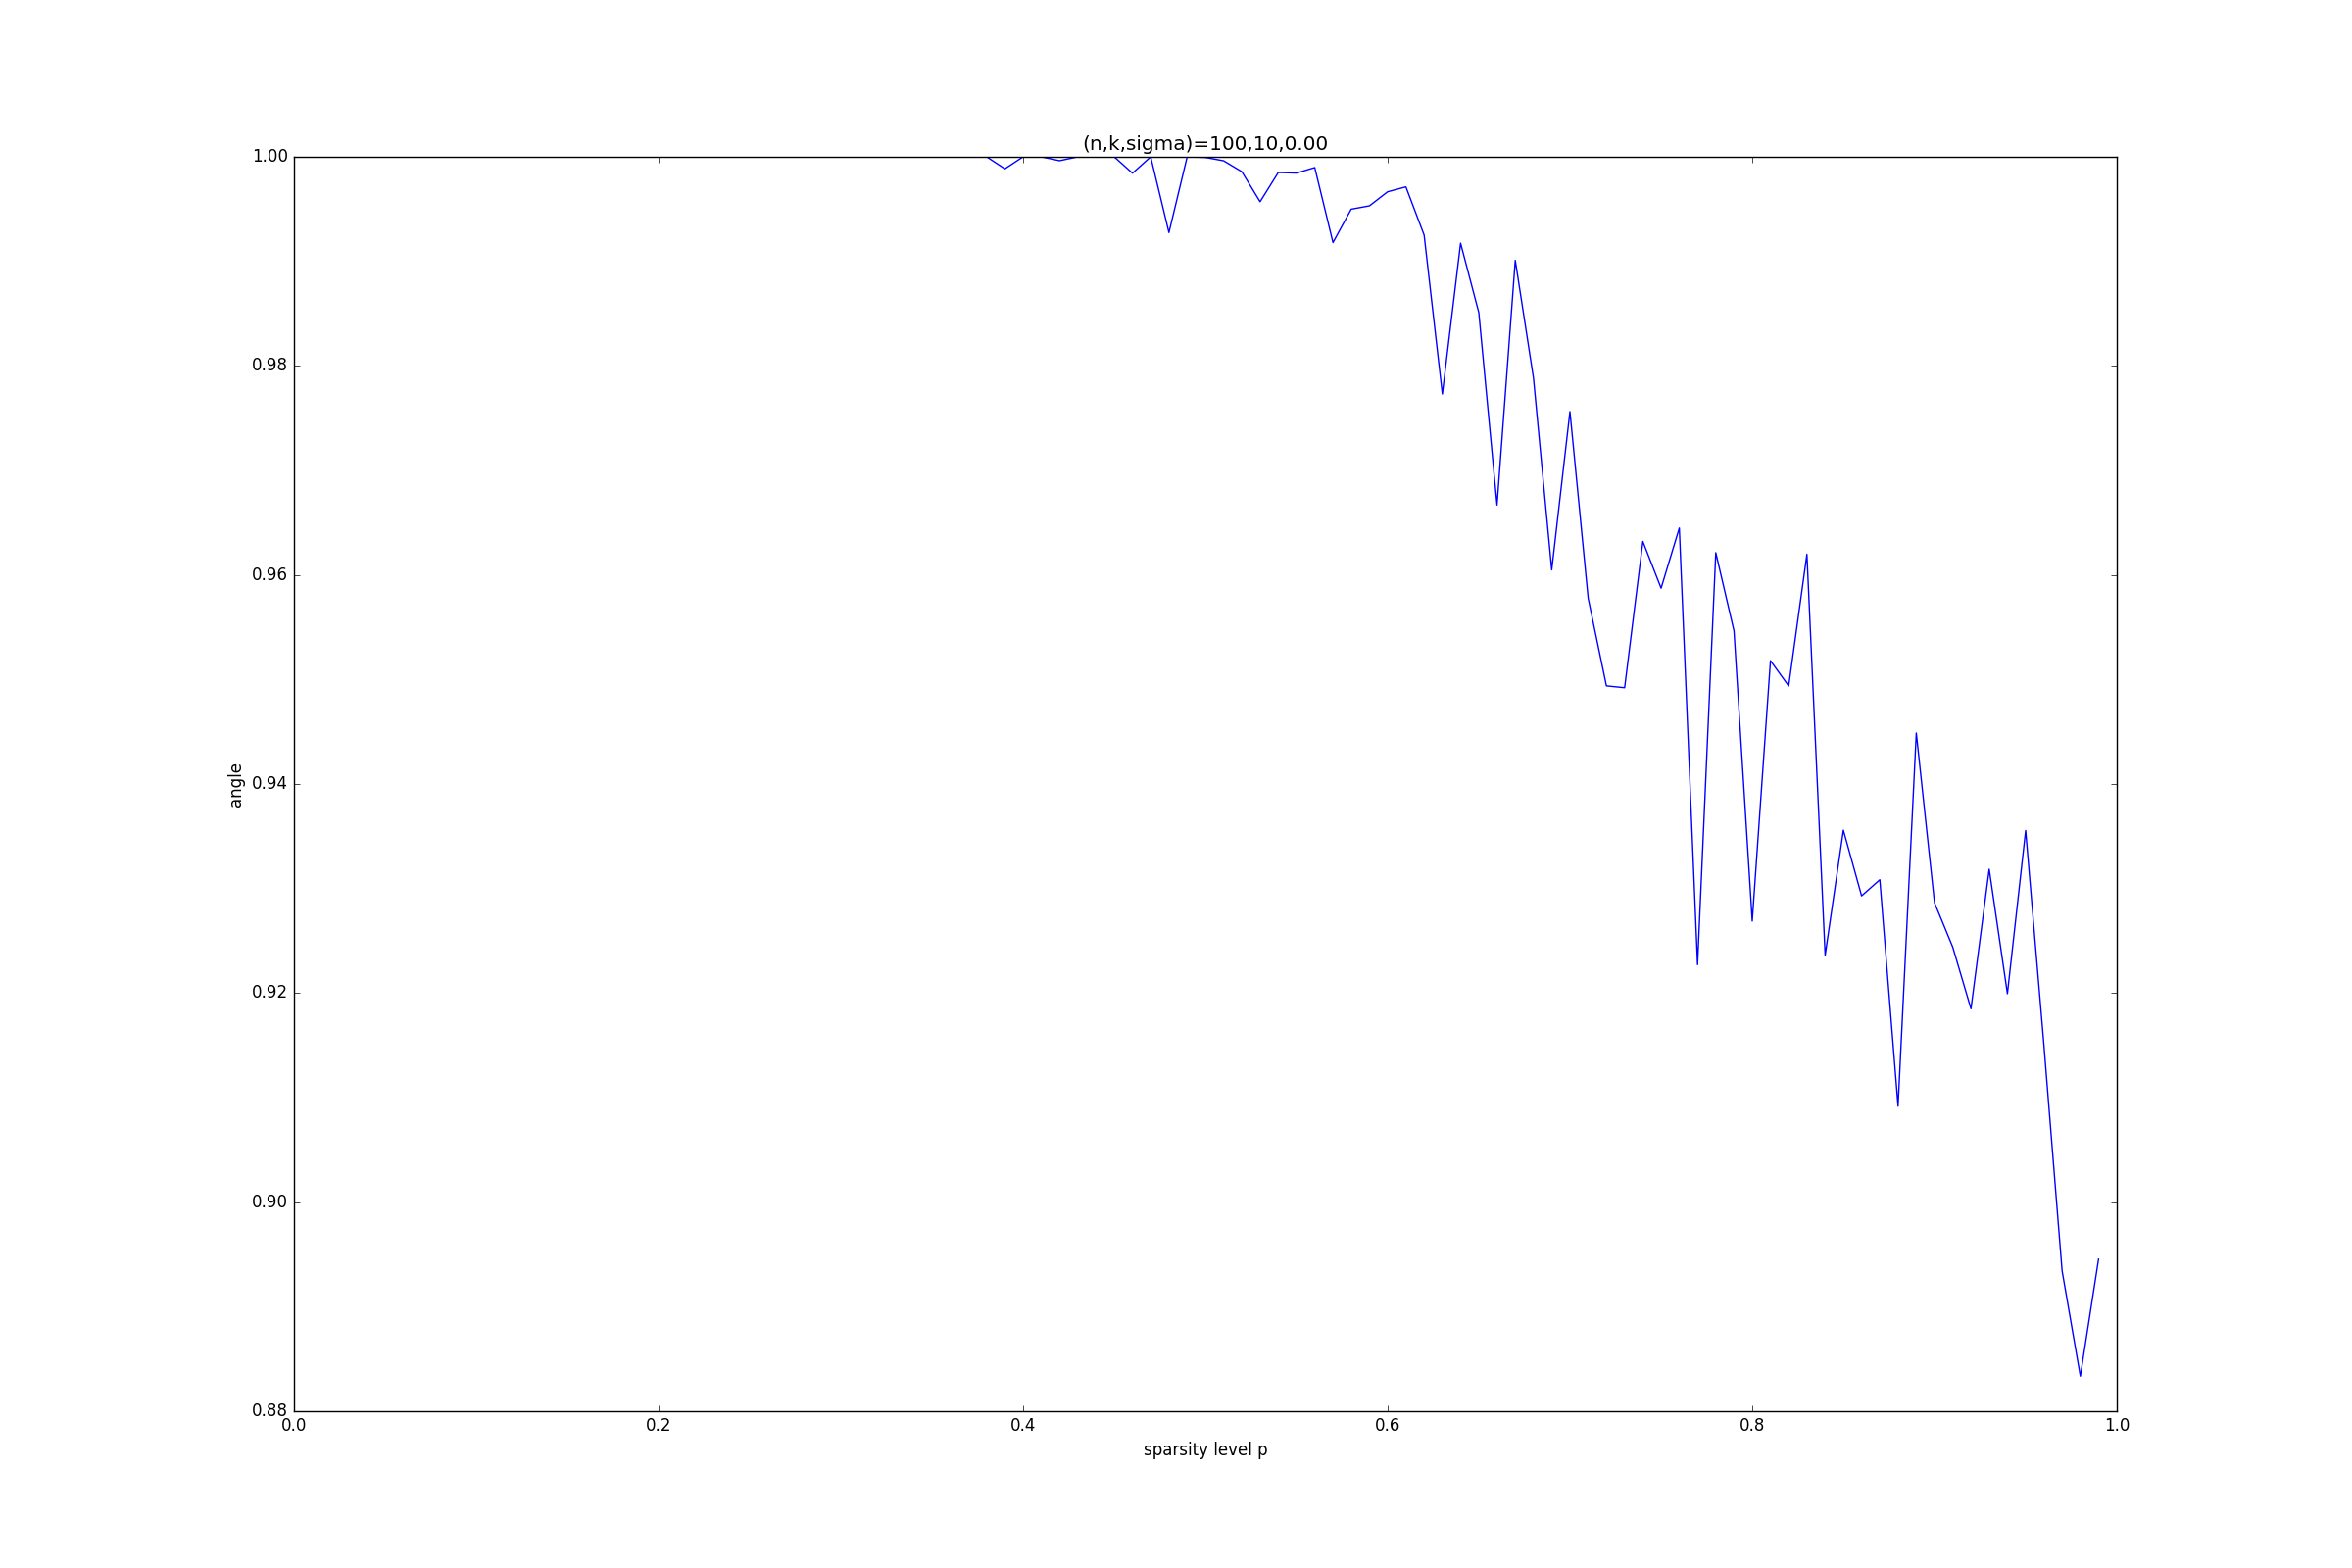
\includegraphics[width=6cm,keepaspectratio]{fig2/w_Norm_x_BerNorm_A_none_n100_k10_p__sigma0_00.png}
 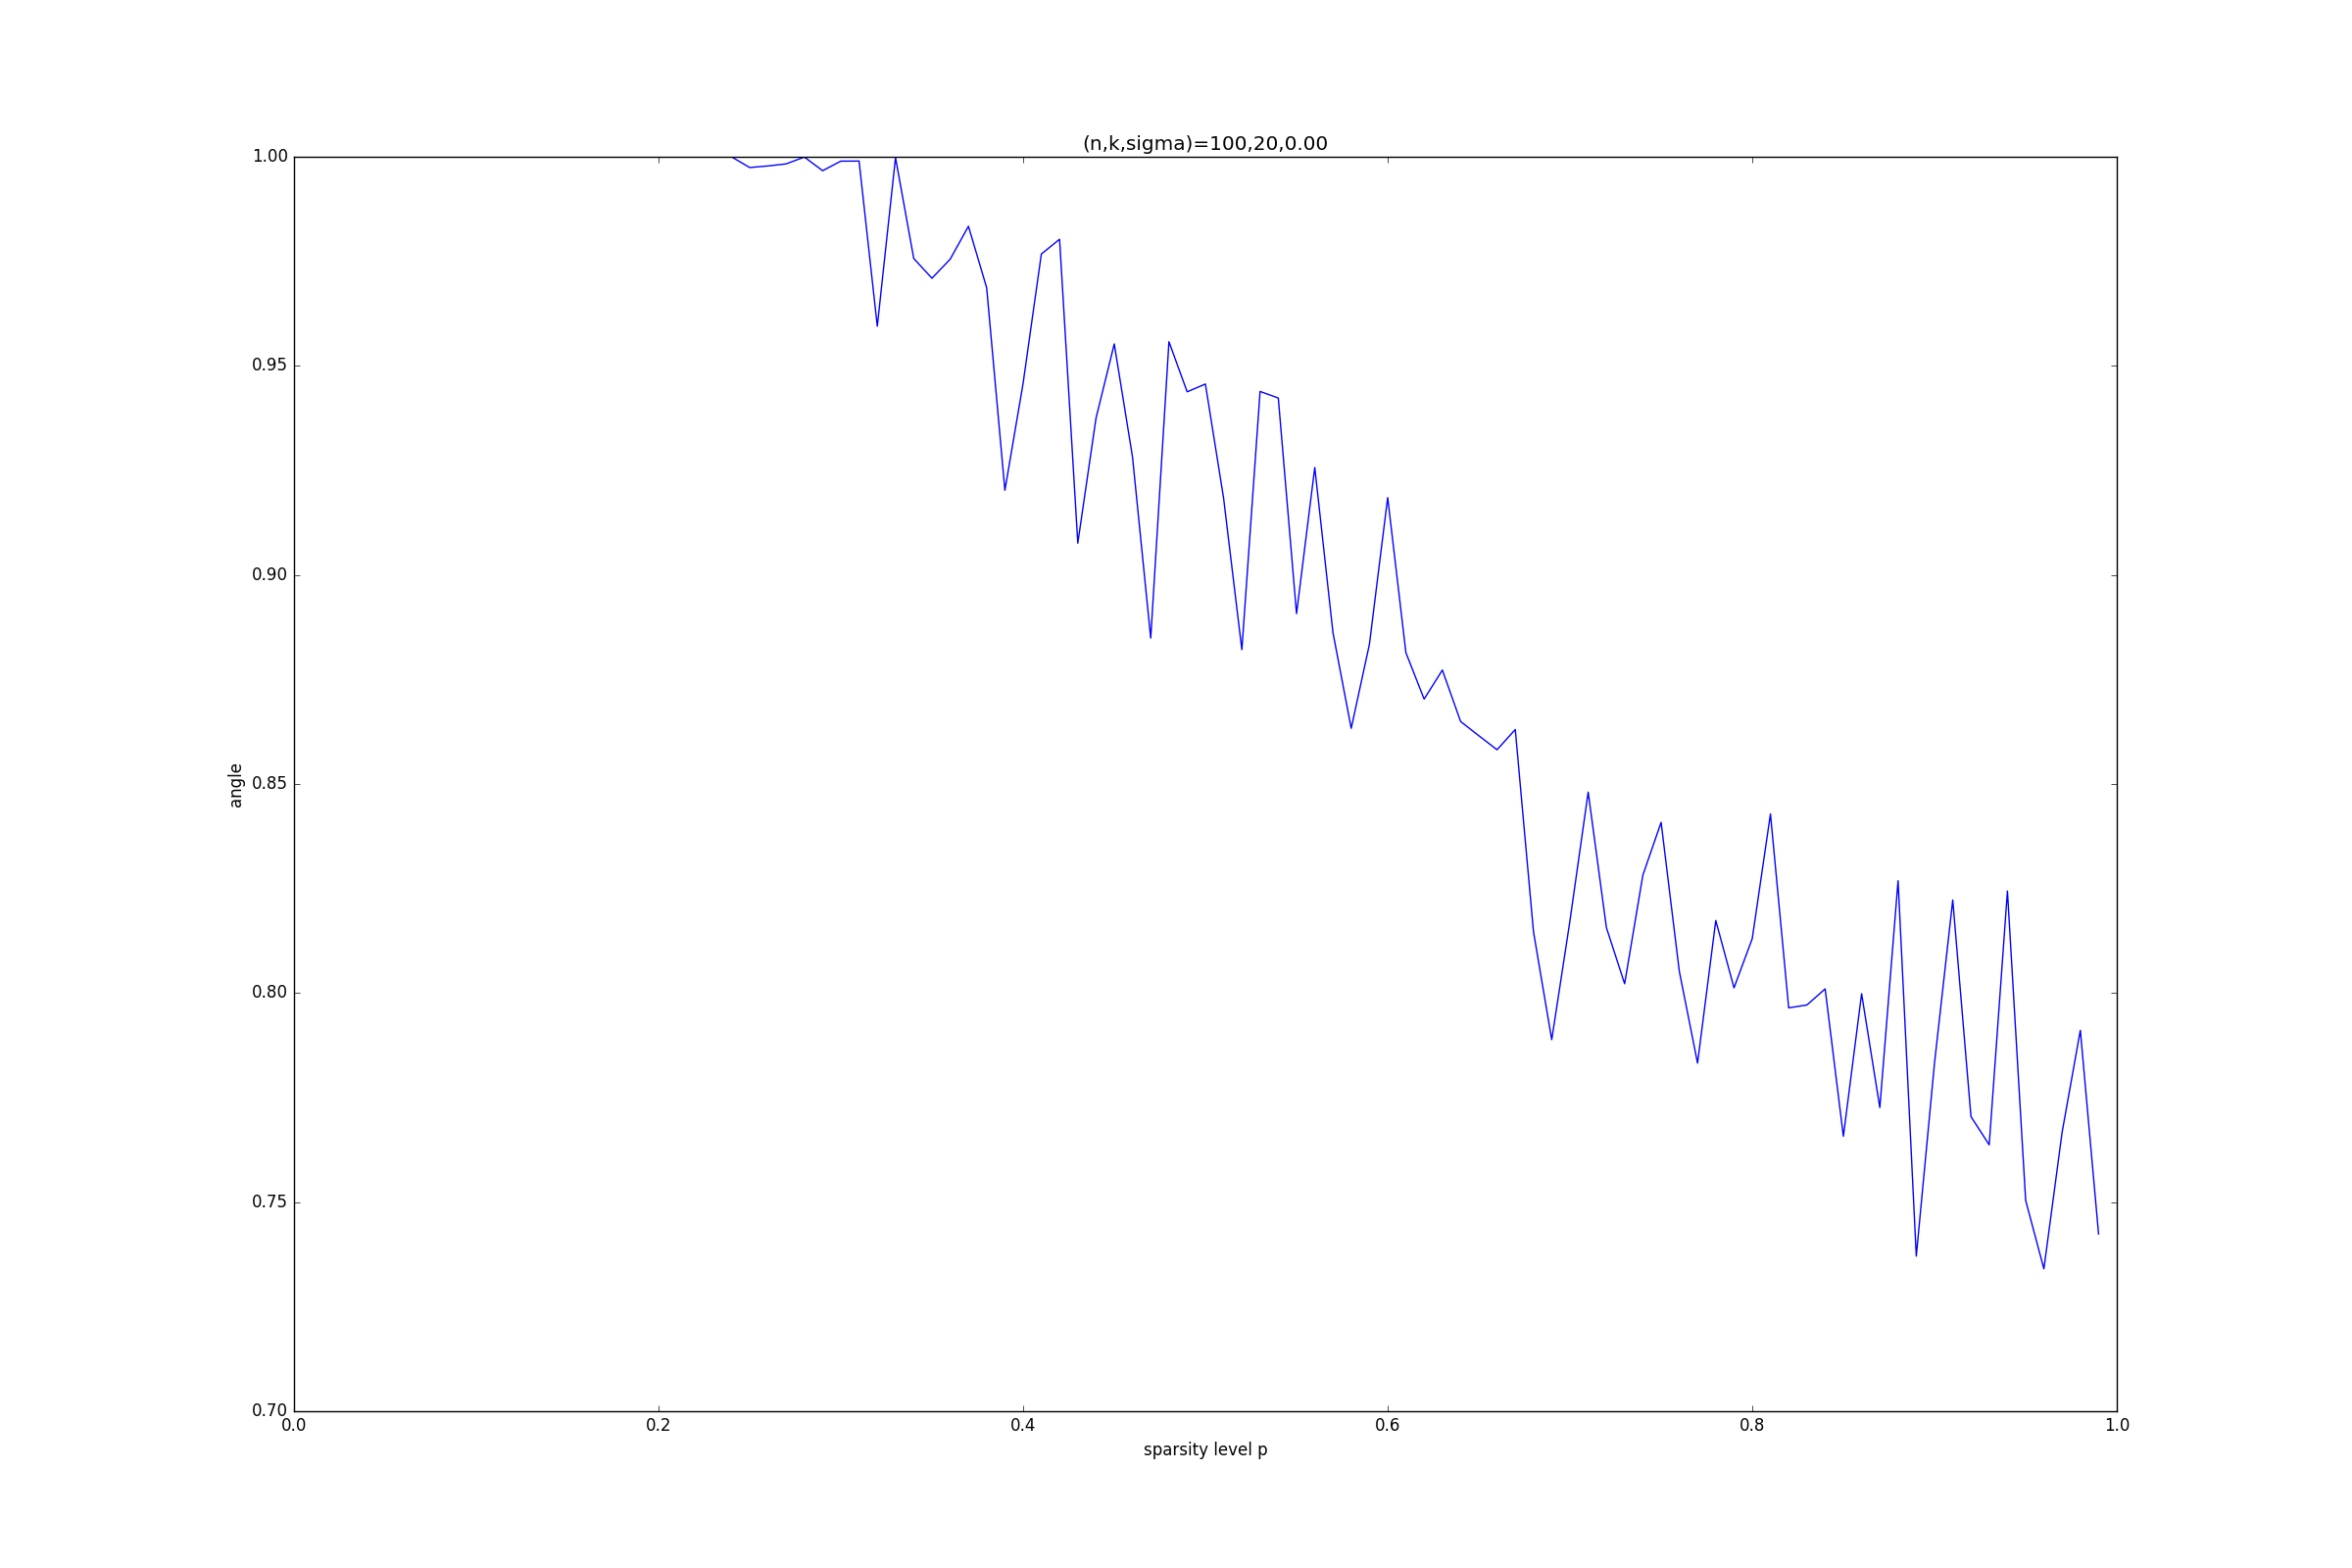
\includegraphics[width=6cm,keepaspectratio]{fig2/w_Norm_x_BerNorm_A_none_n100_k20_p__sigma0_00.png}
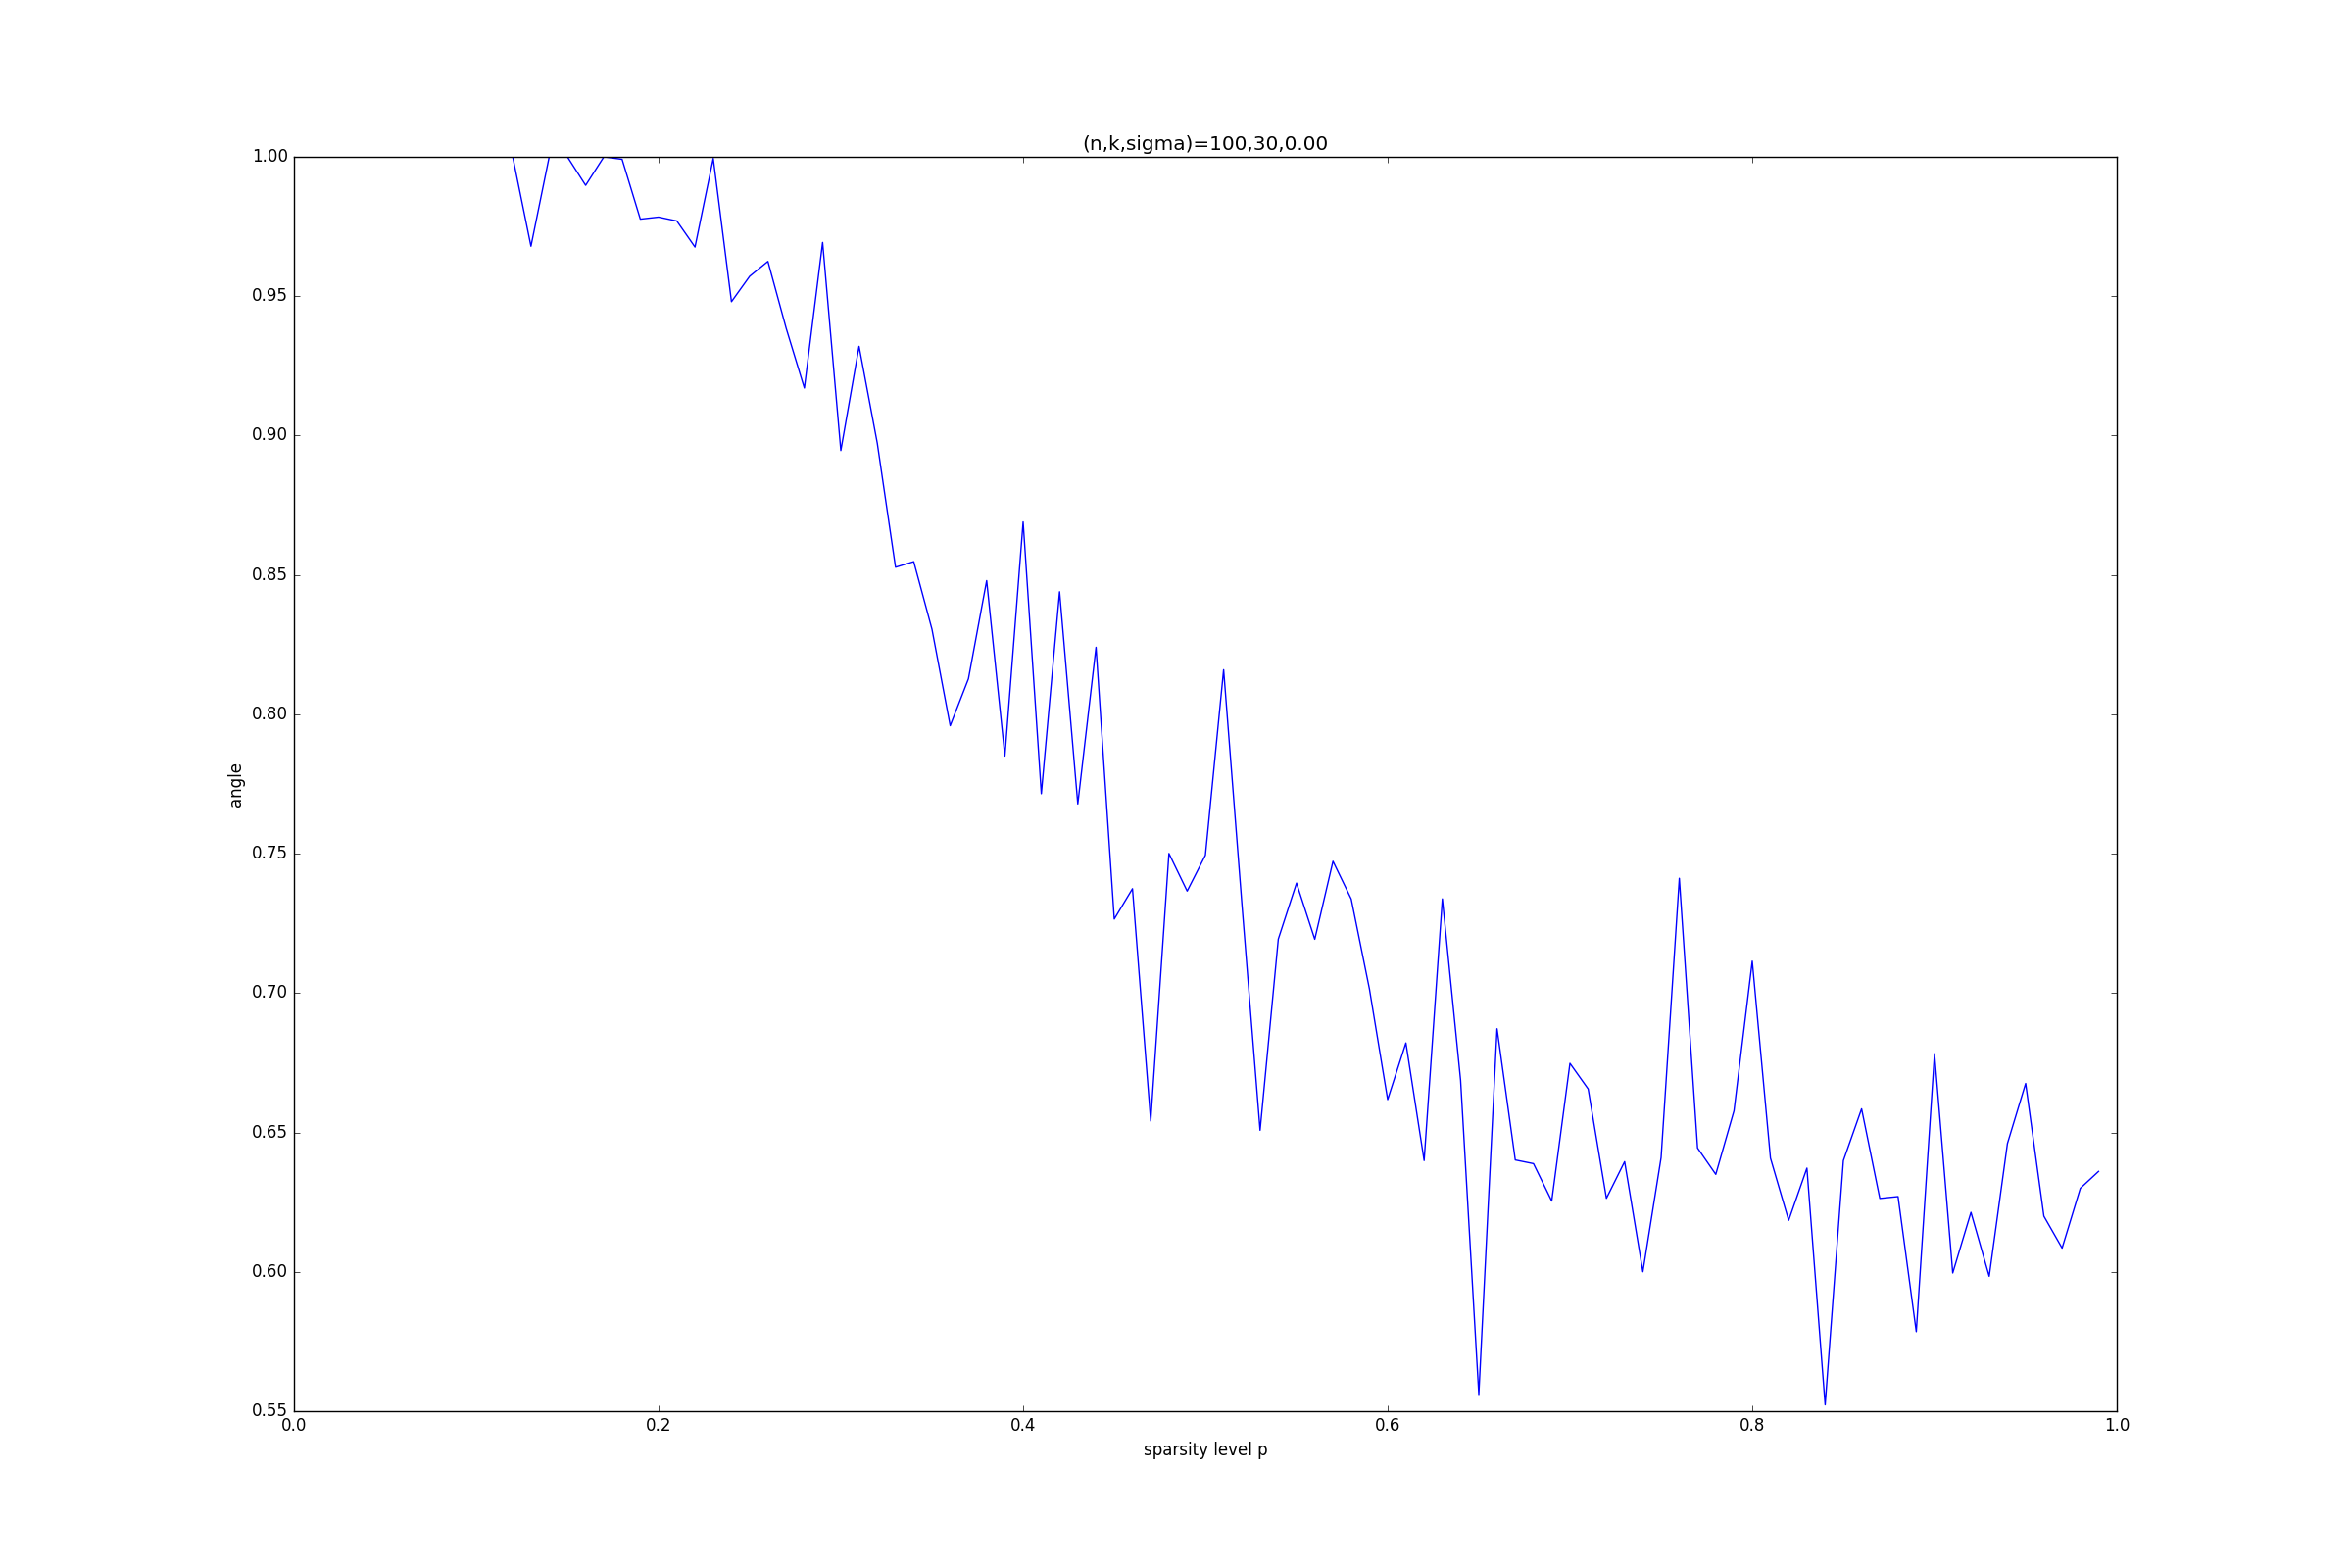
\includegraphics[width=6cm,keepaspectratio]{fig2/w_Norm_x_BerNorm_A_none_n100_k30_p__sigma0_00.png}
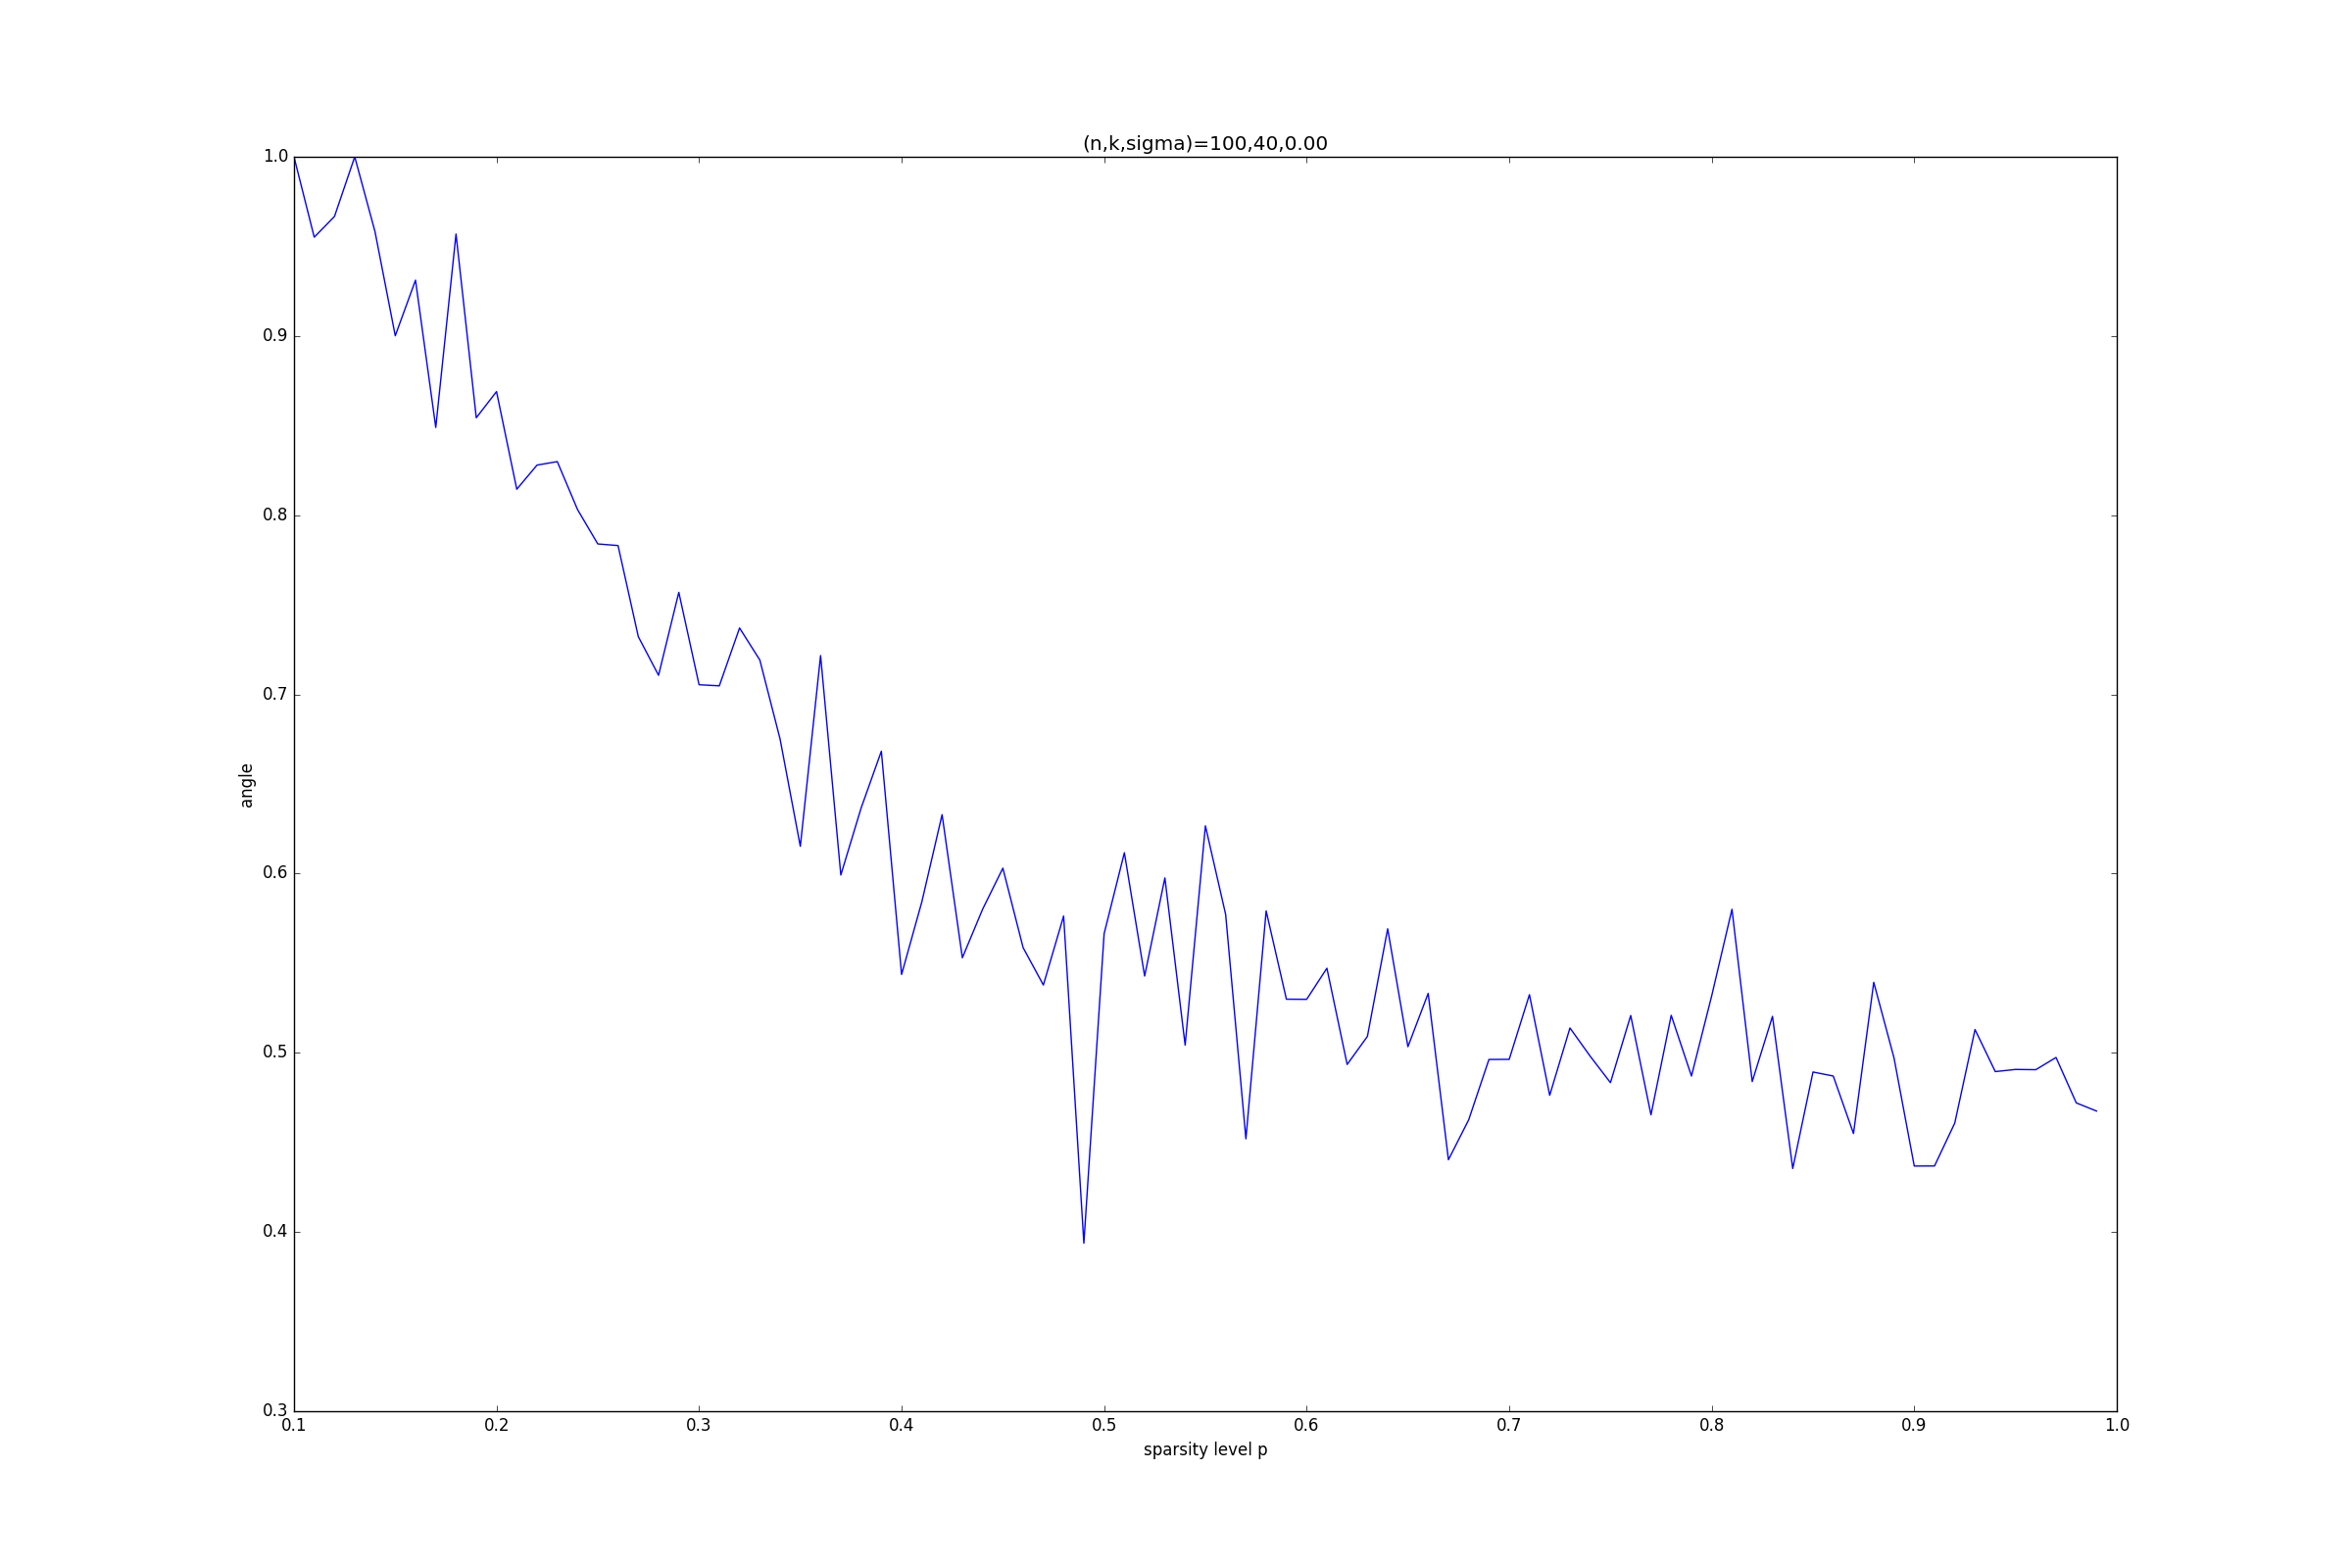
\includegraphics[width=6cm,keepaspectratio]{fig2/w_Norm_x_BerNorm_A_none_n100_k40_p__sigma0_00.png}
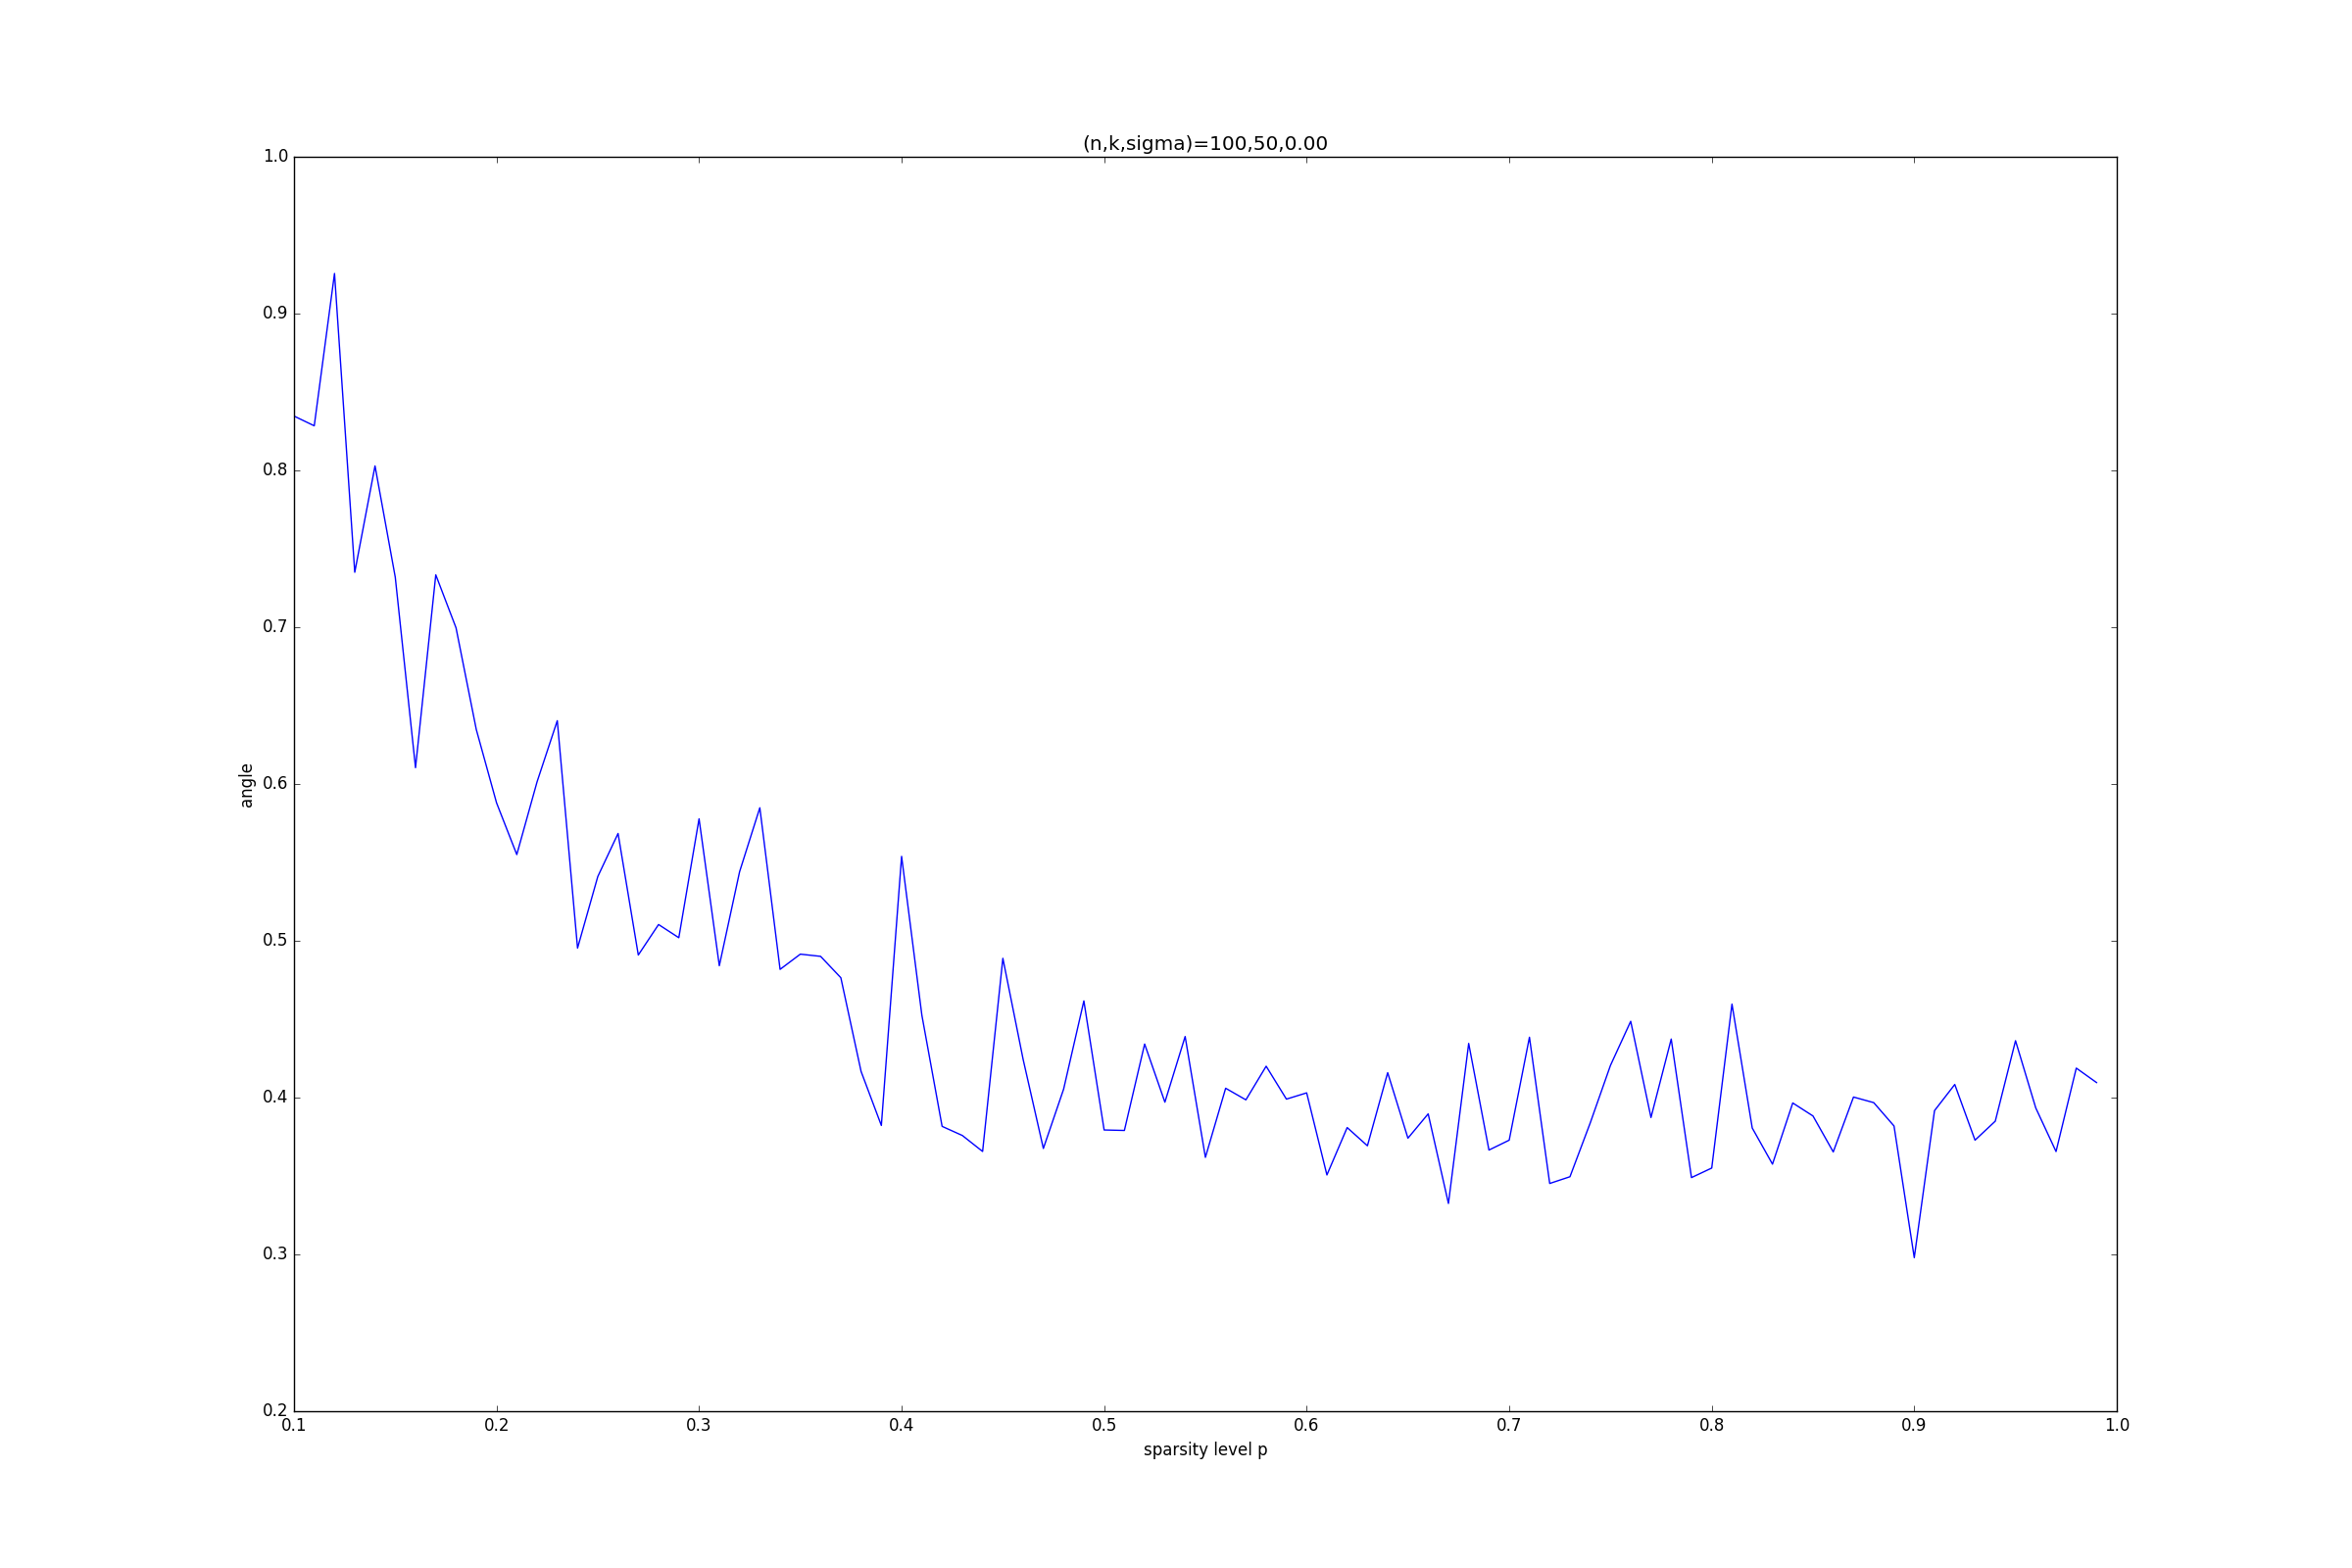
\includegraphics[width=6cm,keepaspectratio]{fig2/w_Norm_x_BerNorm_A_none_n100_k50_p__sigma0_00.png}
\caption{The angle between the estimated $x$ and the ground truth at $k=10, 20, 30, 40, 50$ for $x$ I.I.D. sampled from product of Bernoulli and normal, $b$ I.I.D. sampled from standard normal of length $k$ and $A$ $n\times n$ Gaussian random matrix.   }
\end{figure}

\begin{figure}
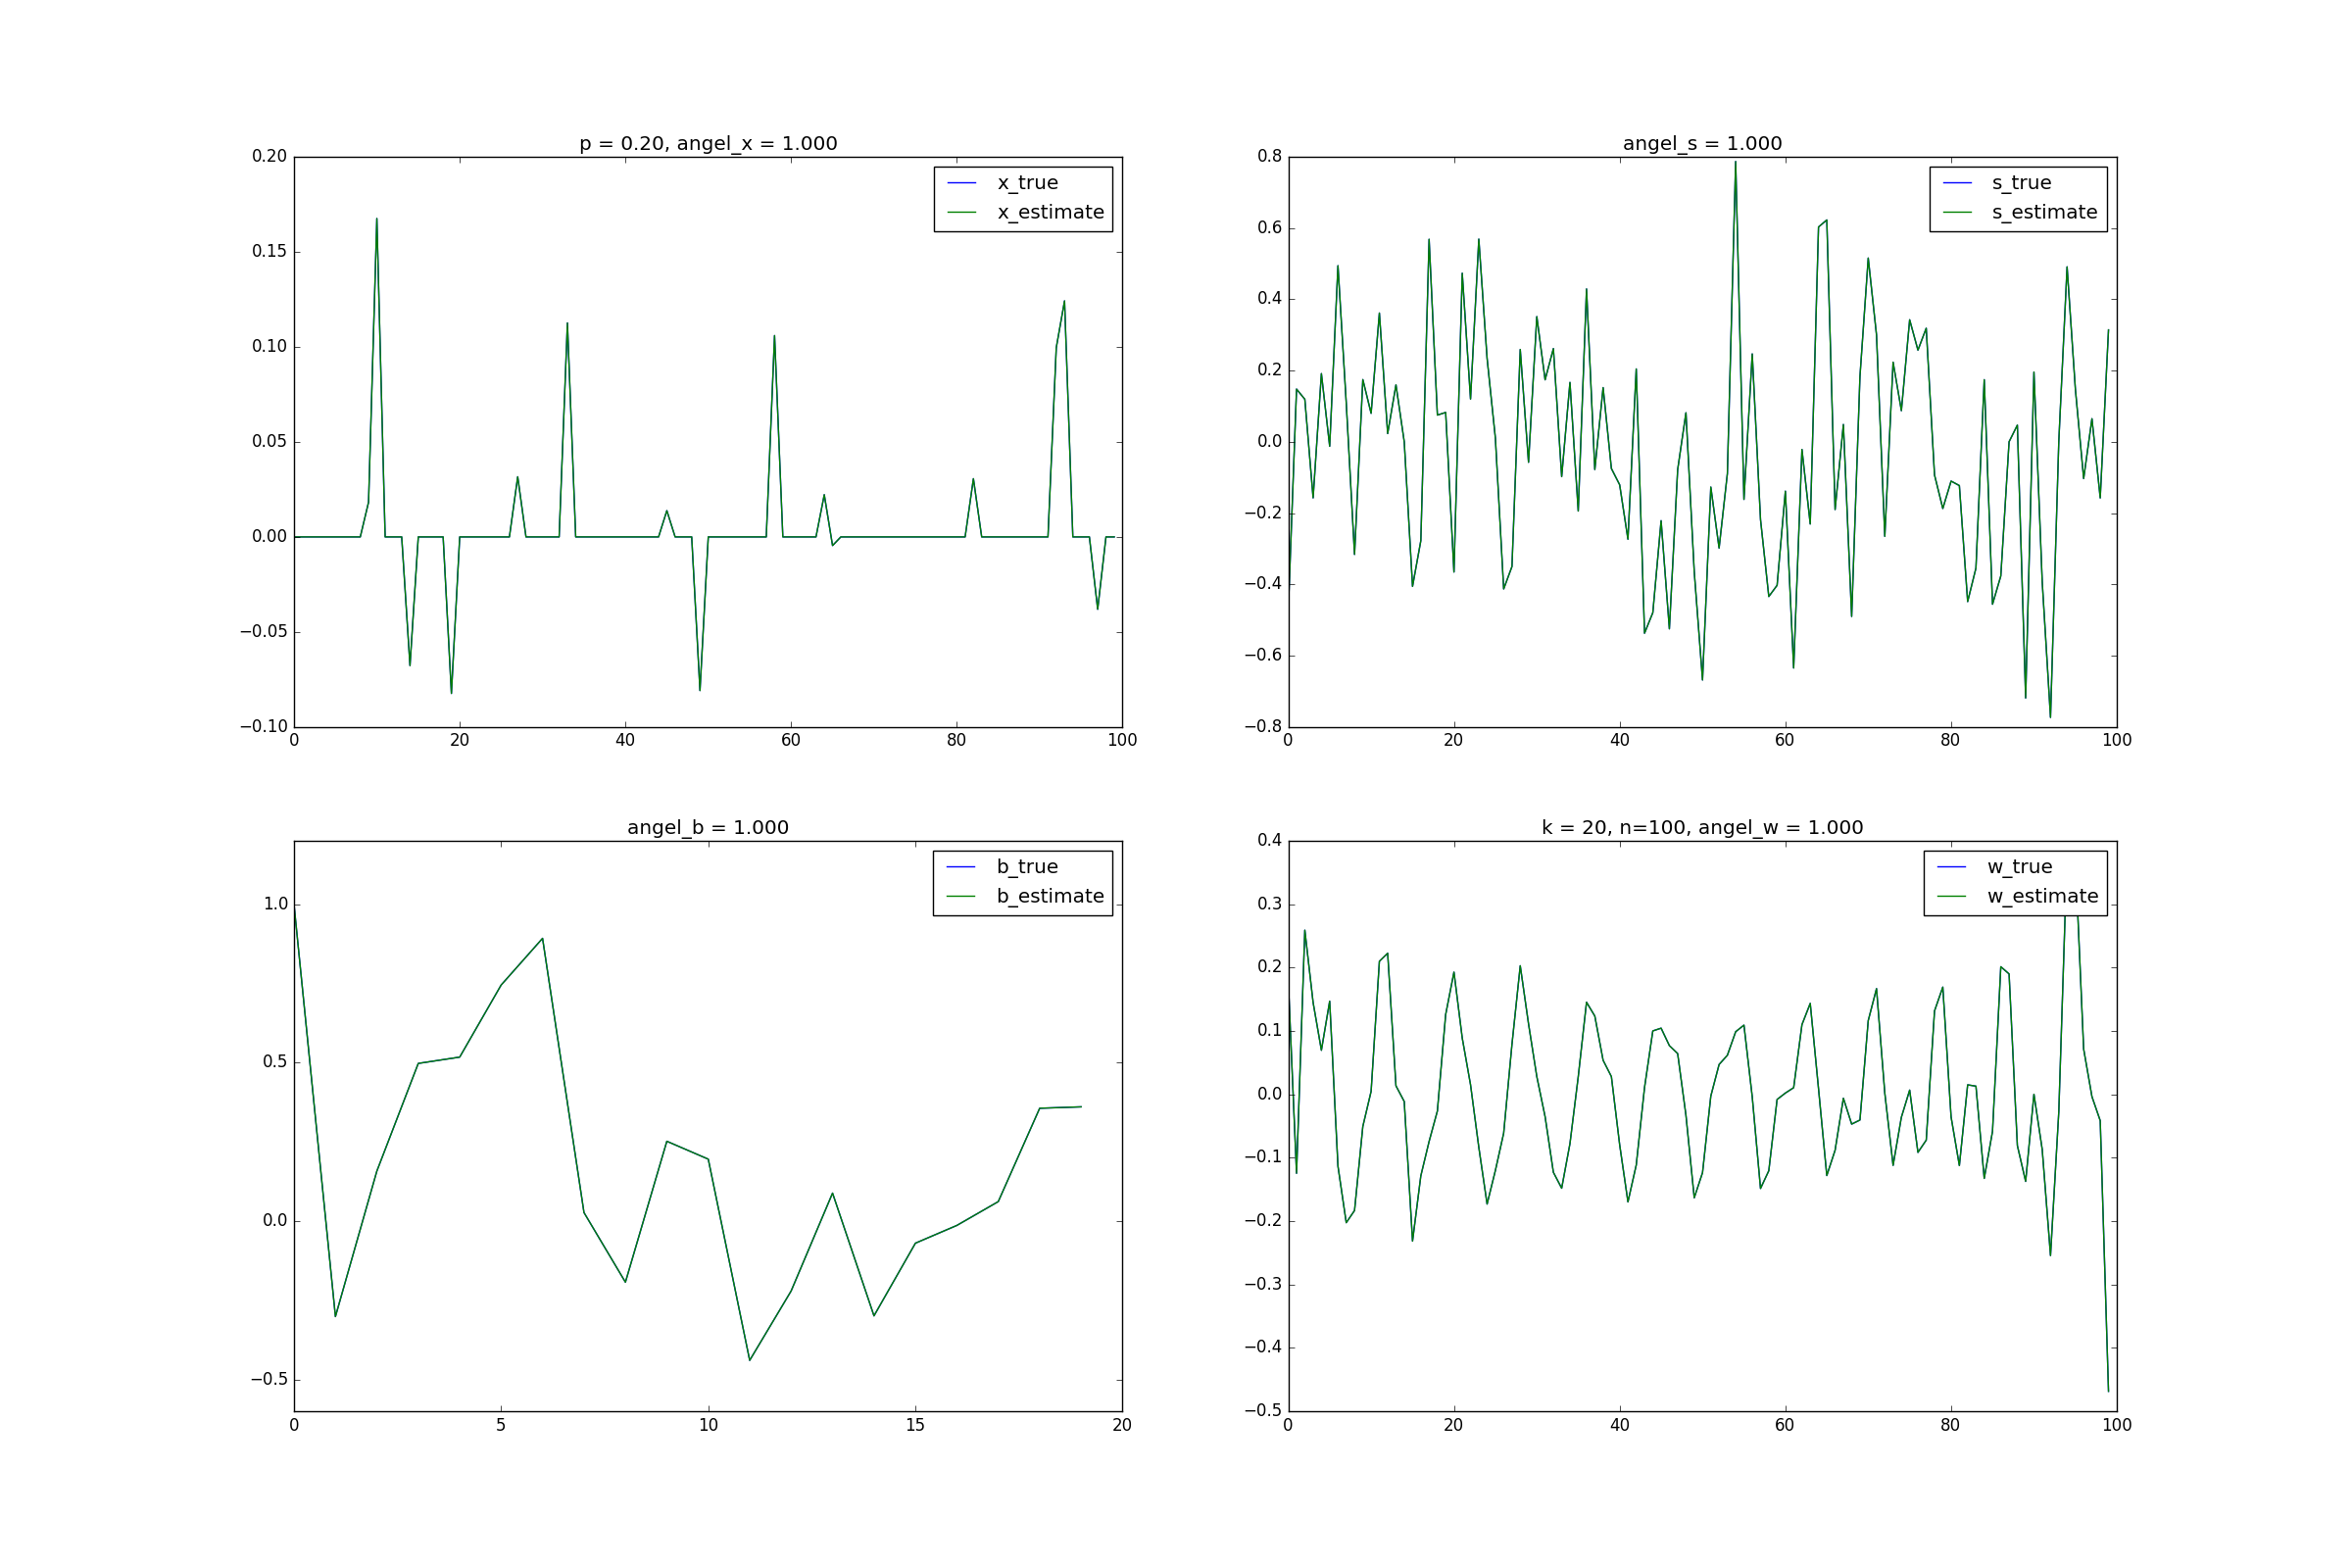
\includegraphics[width=5cm,keepaspectratio]{fig2/04_bShort_k_40_len_xSparse_w_Gaus_AGauss_n100_k20_p0_20_sigma0_00.png}
 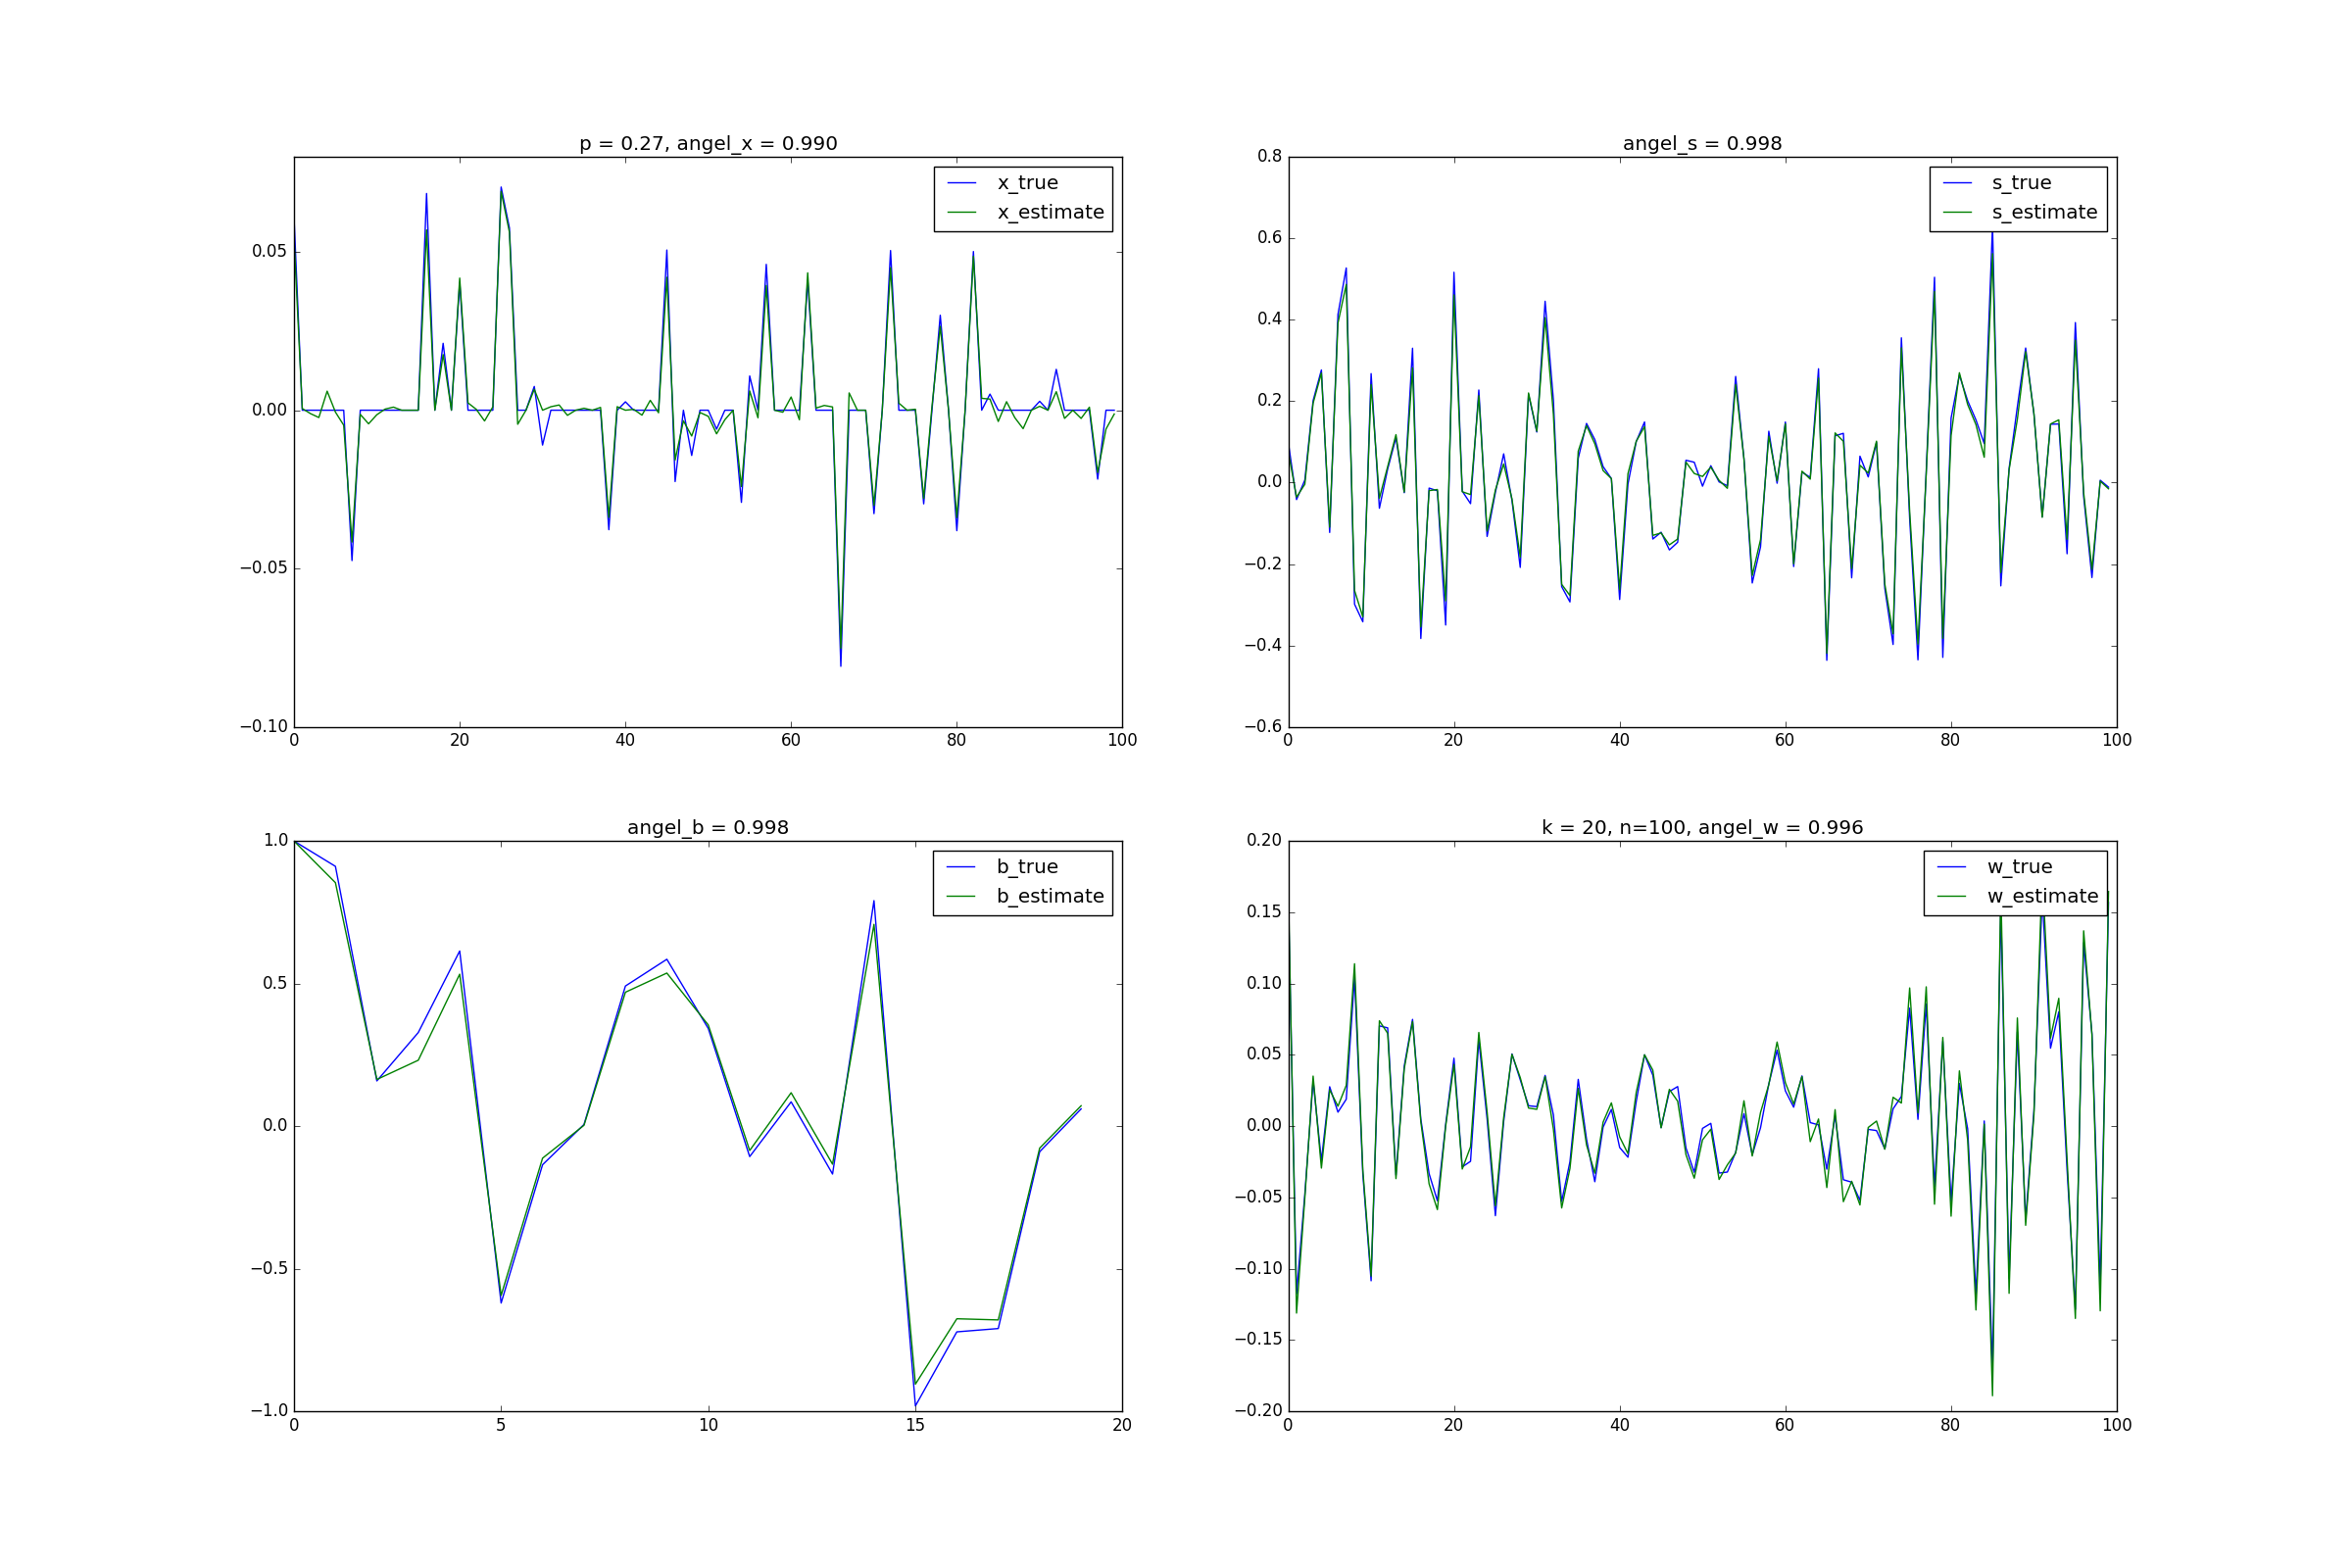
\includegraphics[width=5cm,keepaspectratio]{fig2/04_bShort_k_40_len_xSparse_w_Gaus_AGauss_n100_k20_p0_27_sigma0_00.png}
\caption{Comparison between the ground truth and the estimation for $k=20, p=0.2, 0.27$, the solution is exact at $p=0.2$, the solution is not exact but very close at $p= 0.27$. }
\end{figure}

\begin{figure}
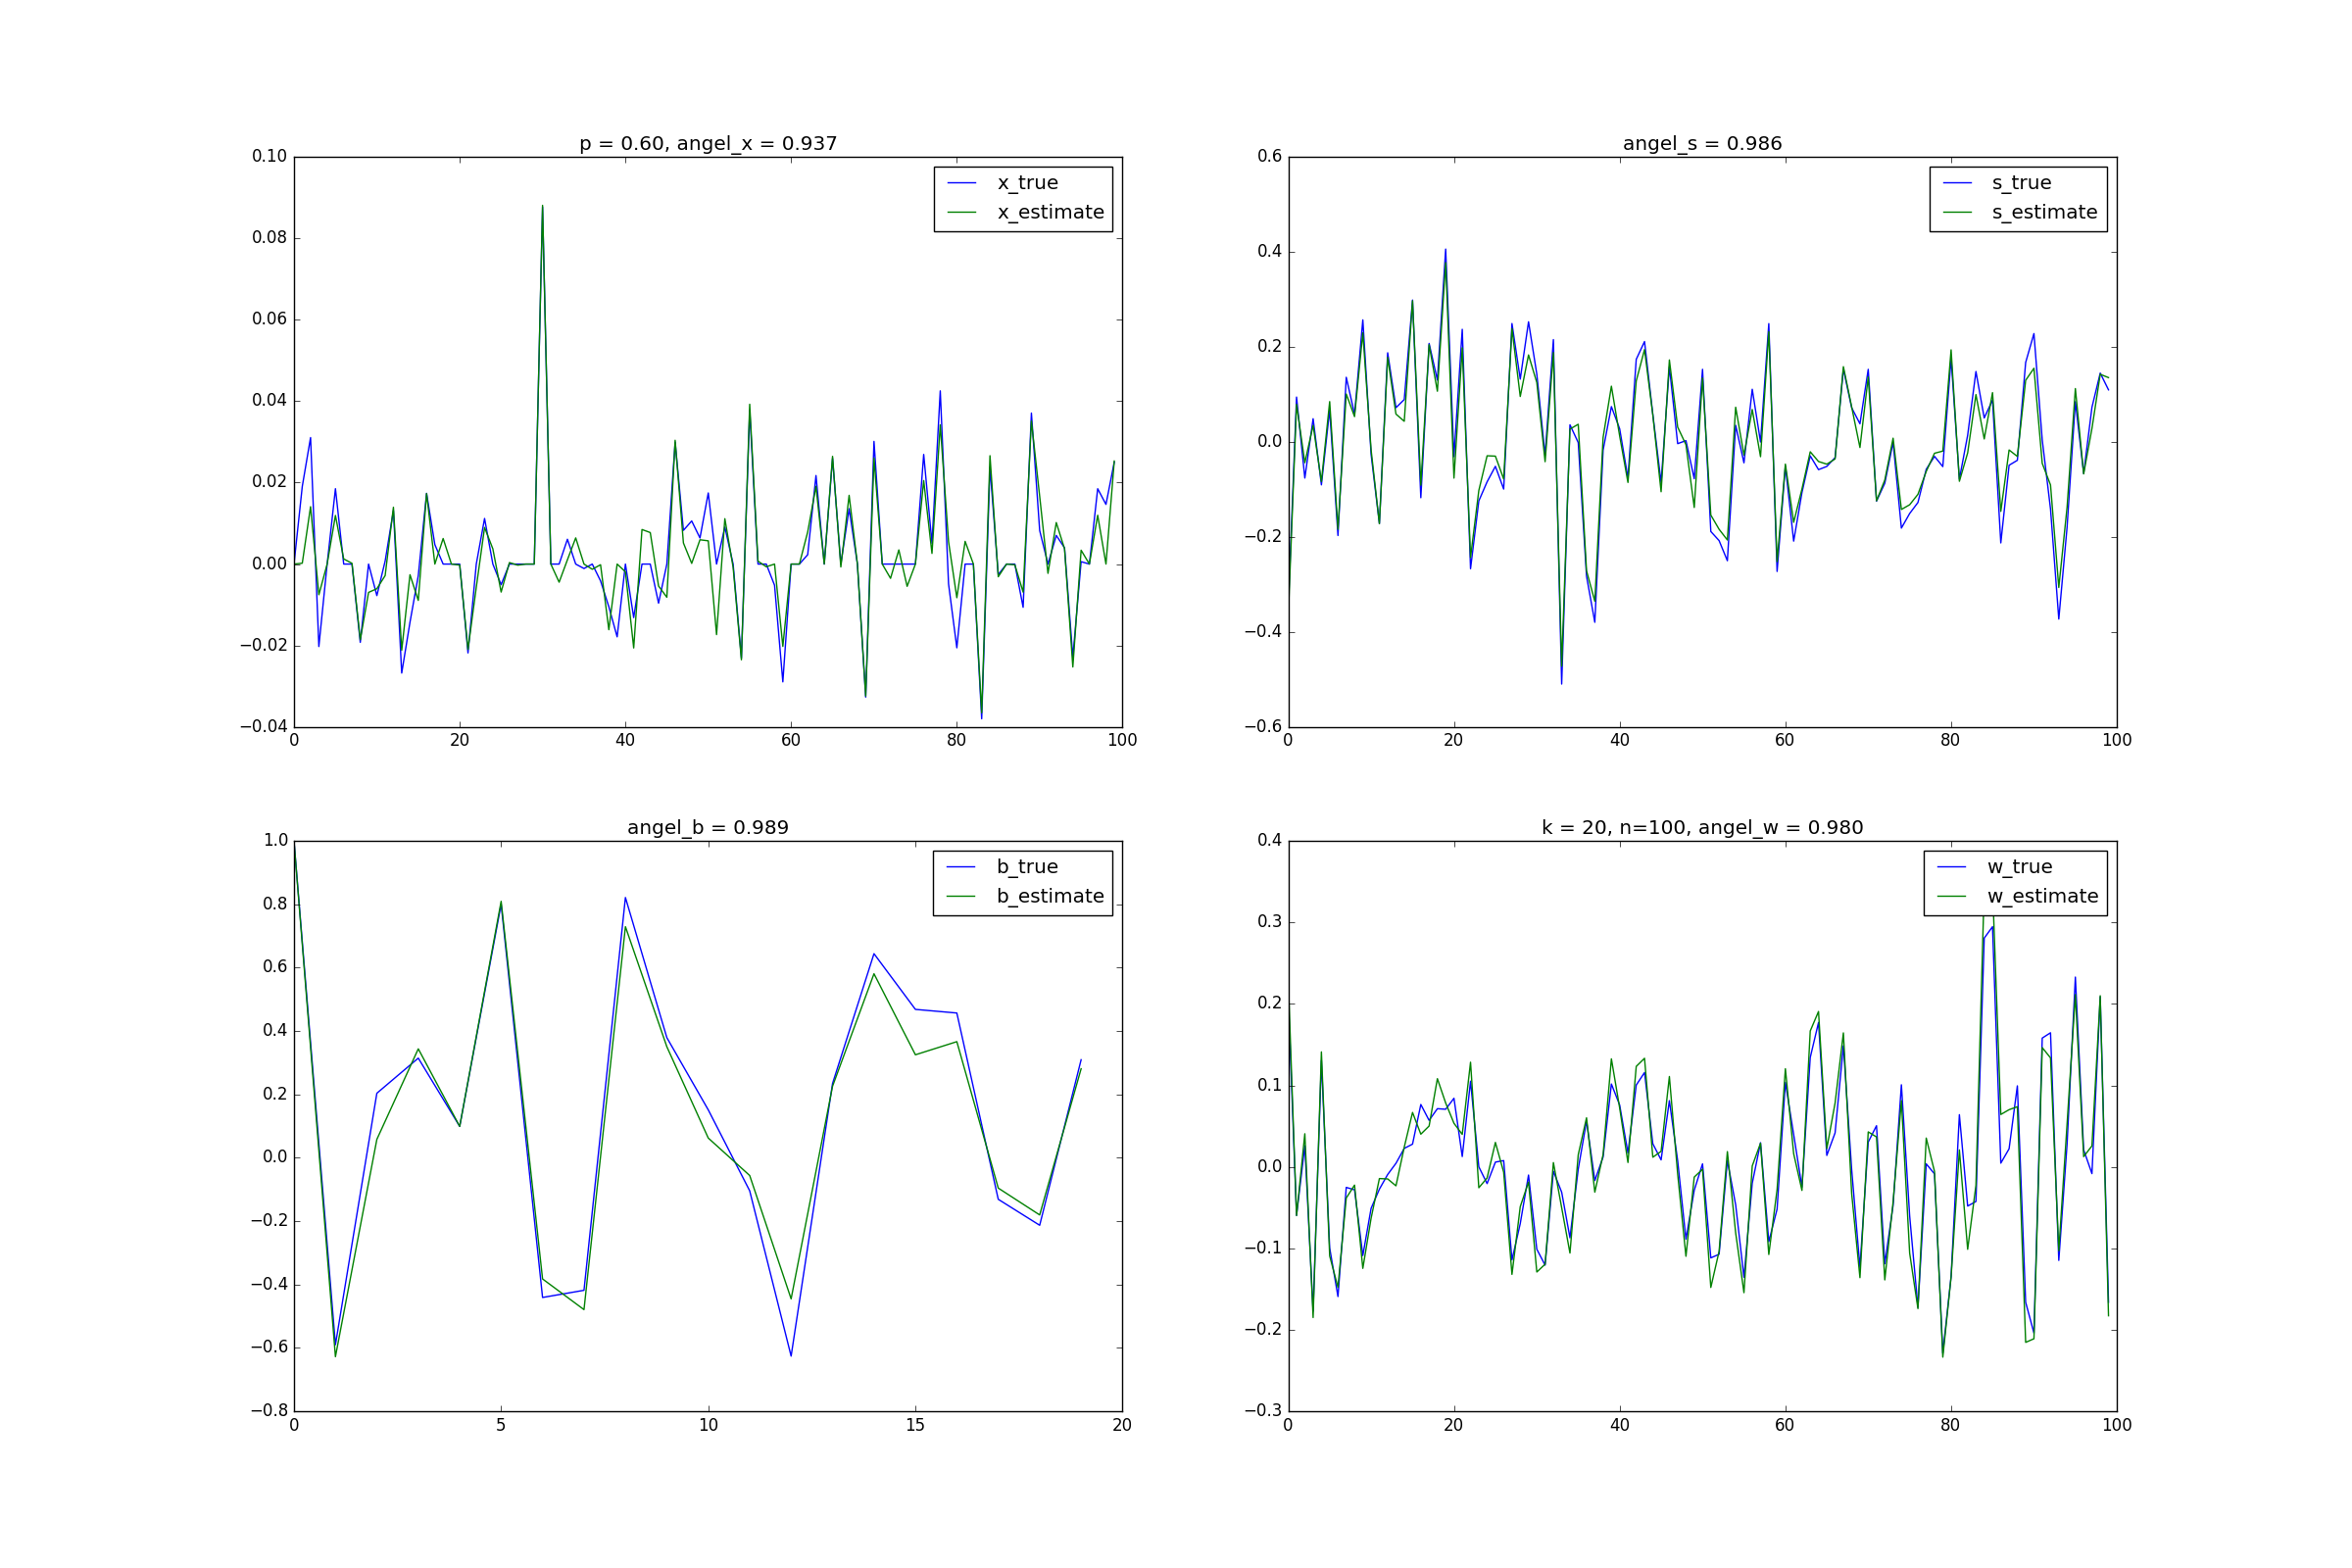
\includegraphics[width=5cm,keepaspectratio]{fig2/bShort_k_lenKnown_xSparse_w_Gaus_AGauss_n100_k20_p0_60_sigma0_00.png}
   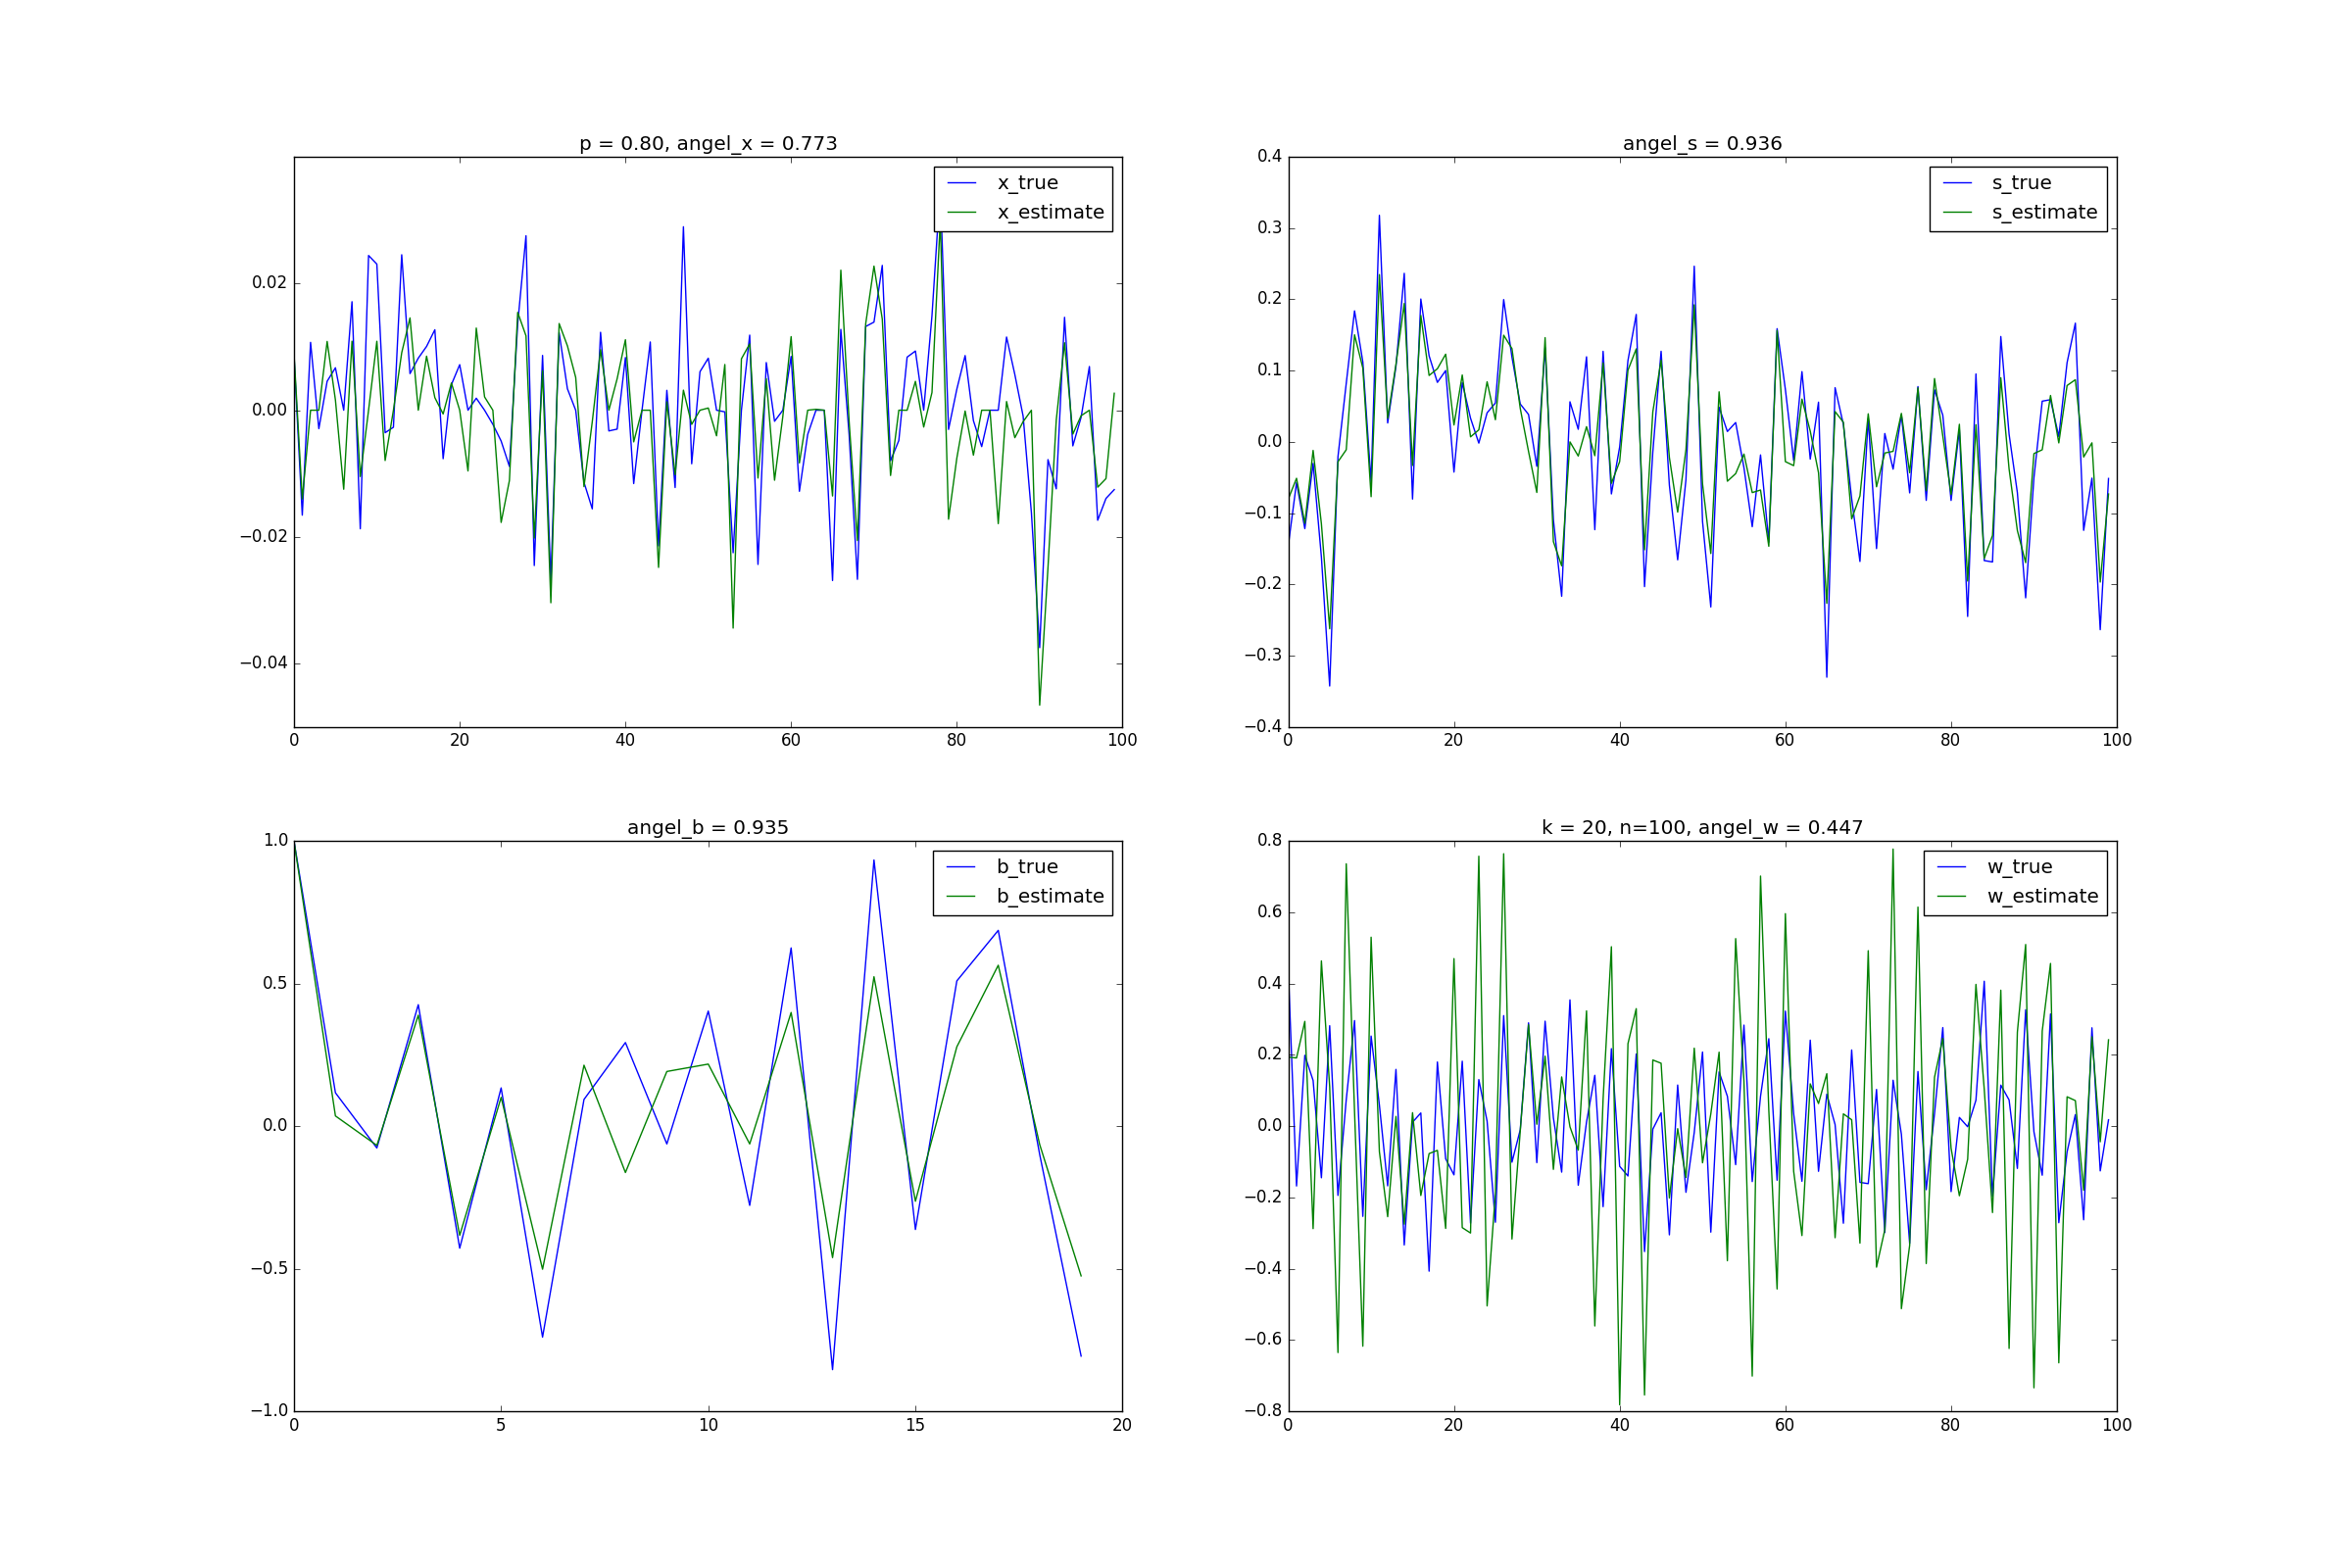
\includegraphics[width=5cm,keepaspectratio]{fig2/bShort_k_lenKnown_xSparse_w_Gaus_AGauss_n100_k20_p0_80_sigma0_00.png}
\caption{Comparison between the ground truth and the estimation for $k=20, p= 0.4, 0.6, 0.8$, the solution is reasonable at $p=0.4, 0.6, 0.8$. }
\end{figure}



\begin{figure}
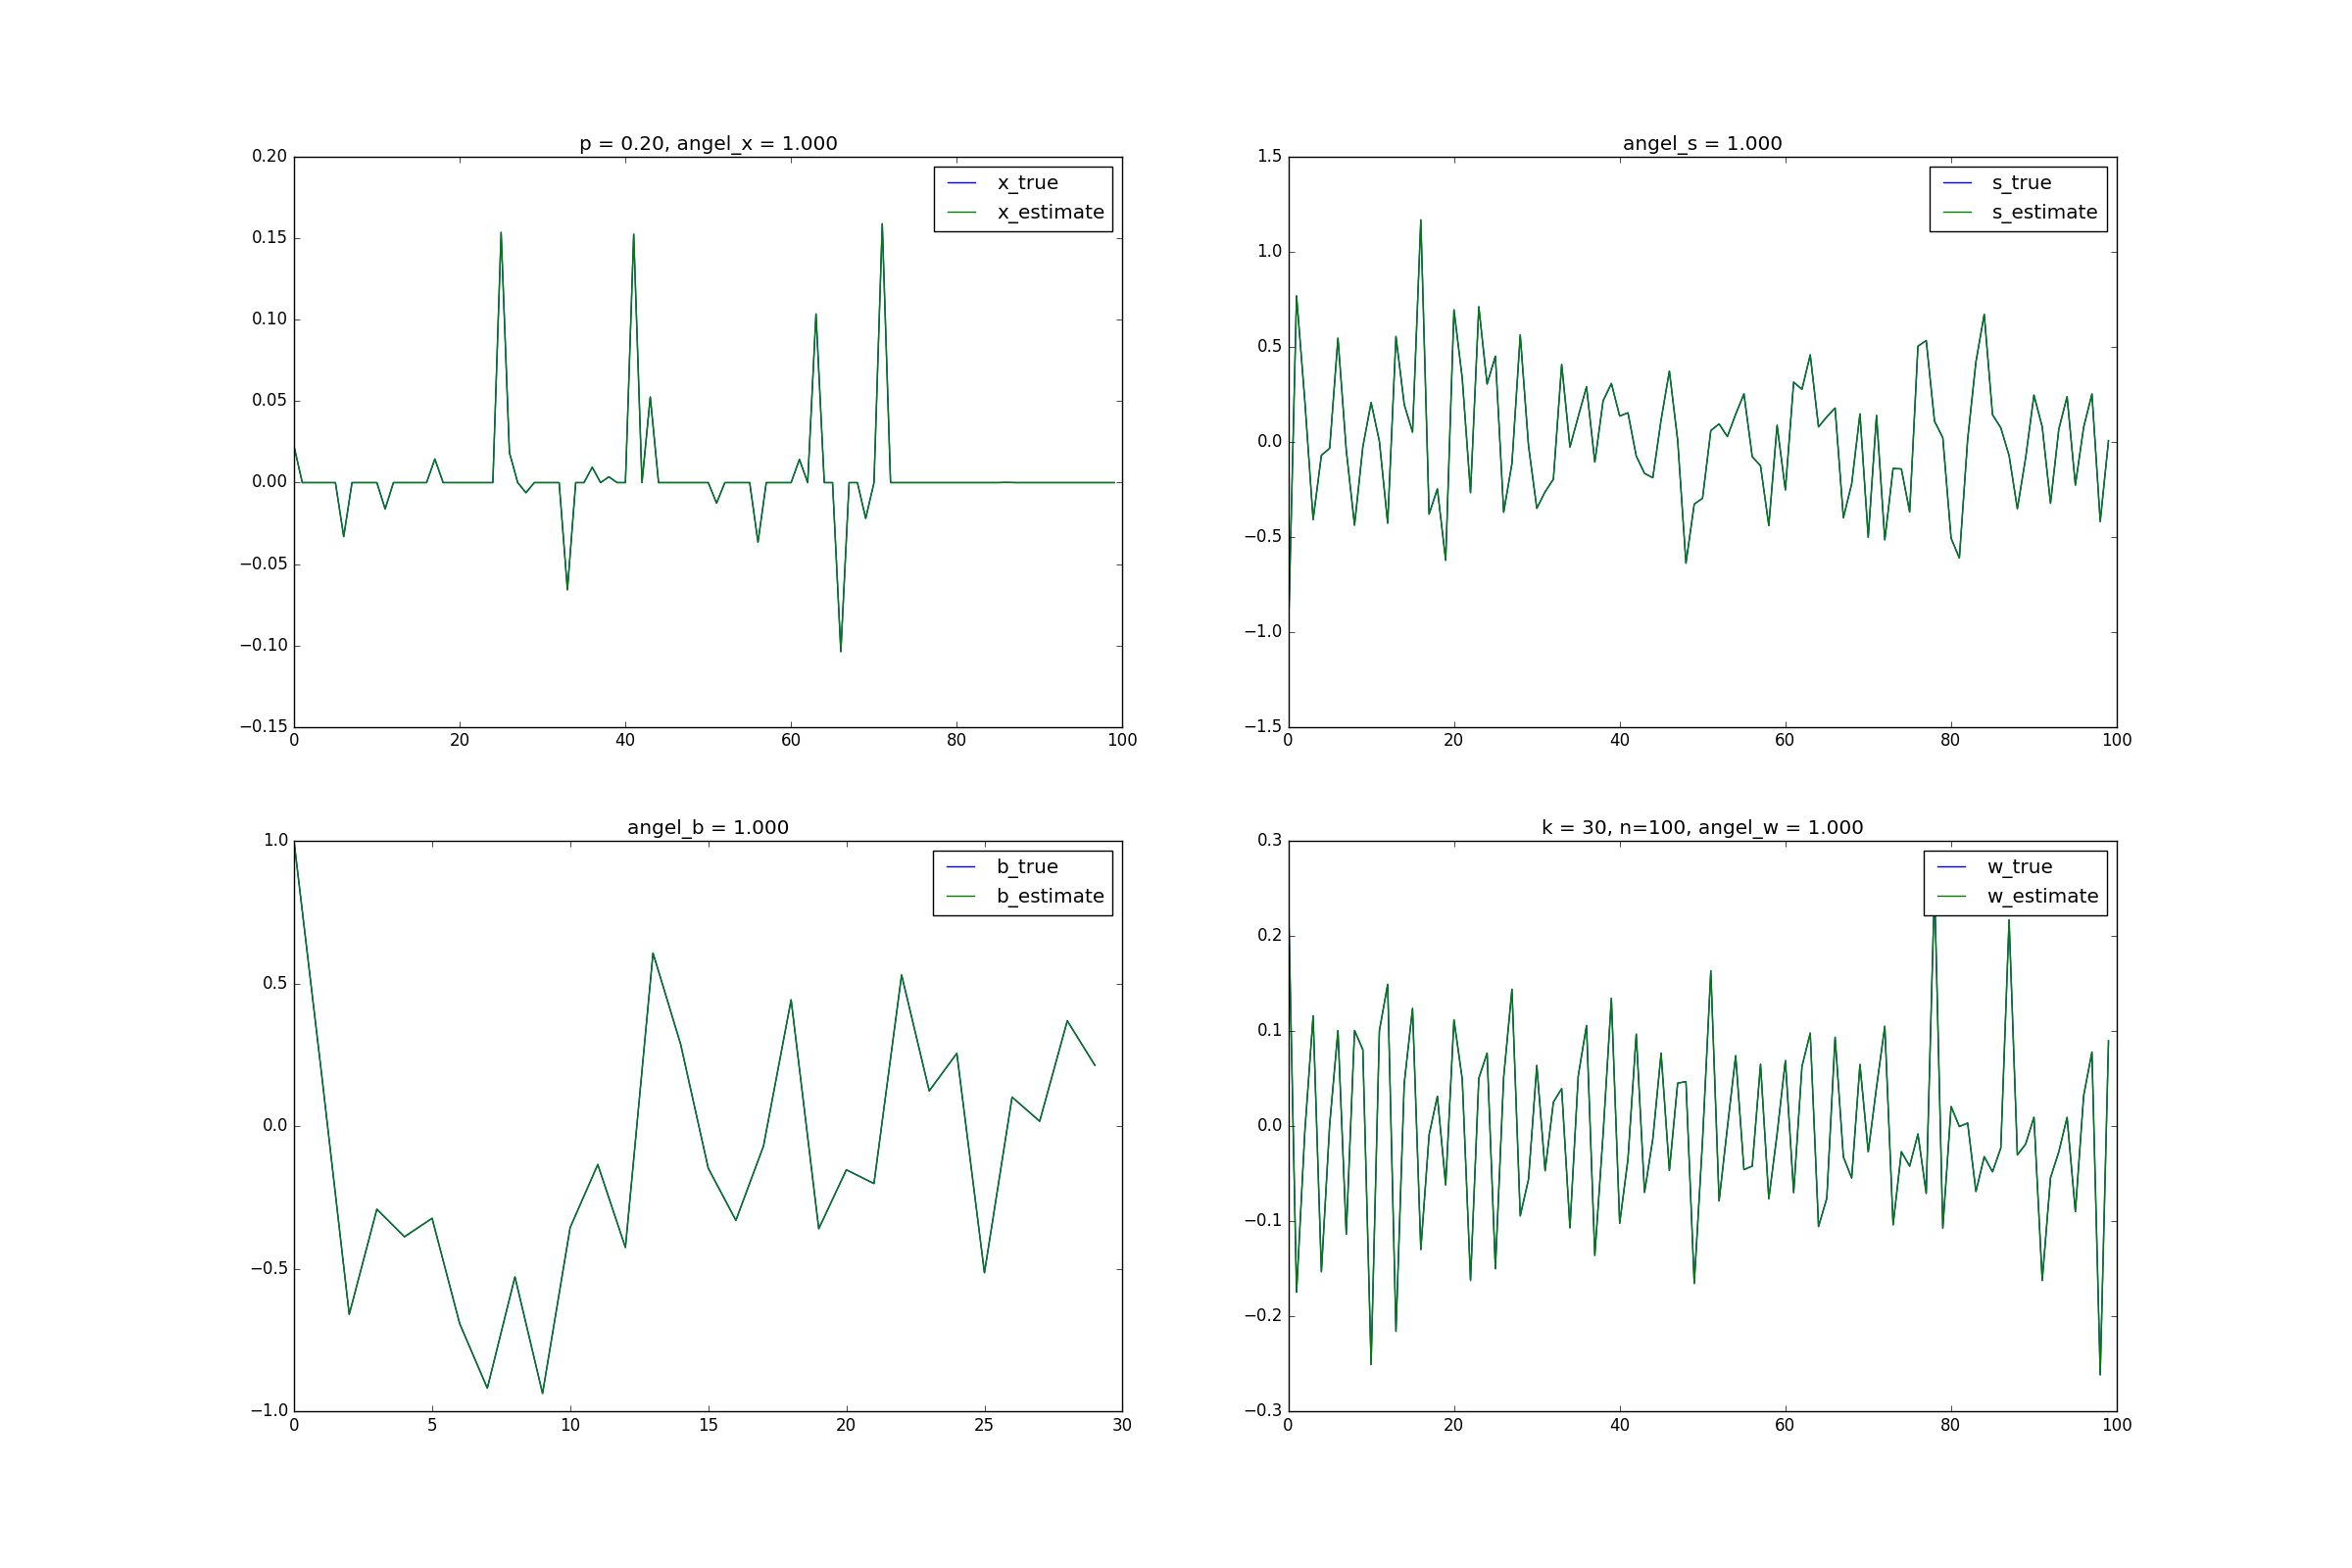
\includegraphics[width=6cm,keepaspectratio]{fig2/bShort_k_lenKnown_xSparse_w_Gaus_AGauss_n100_k30_p0_20_sigma0_00.png}
 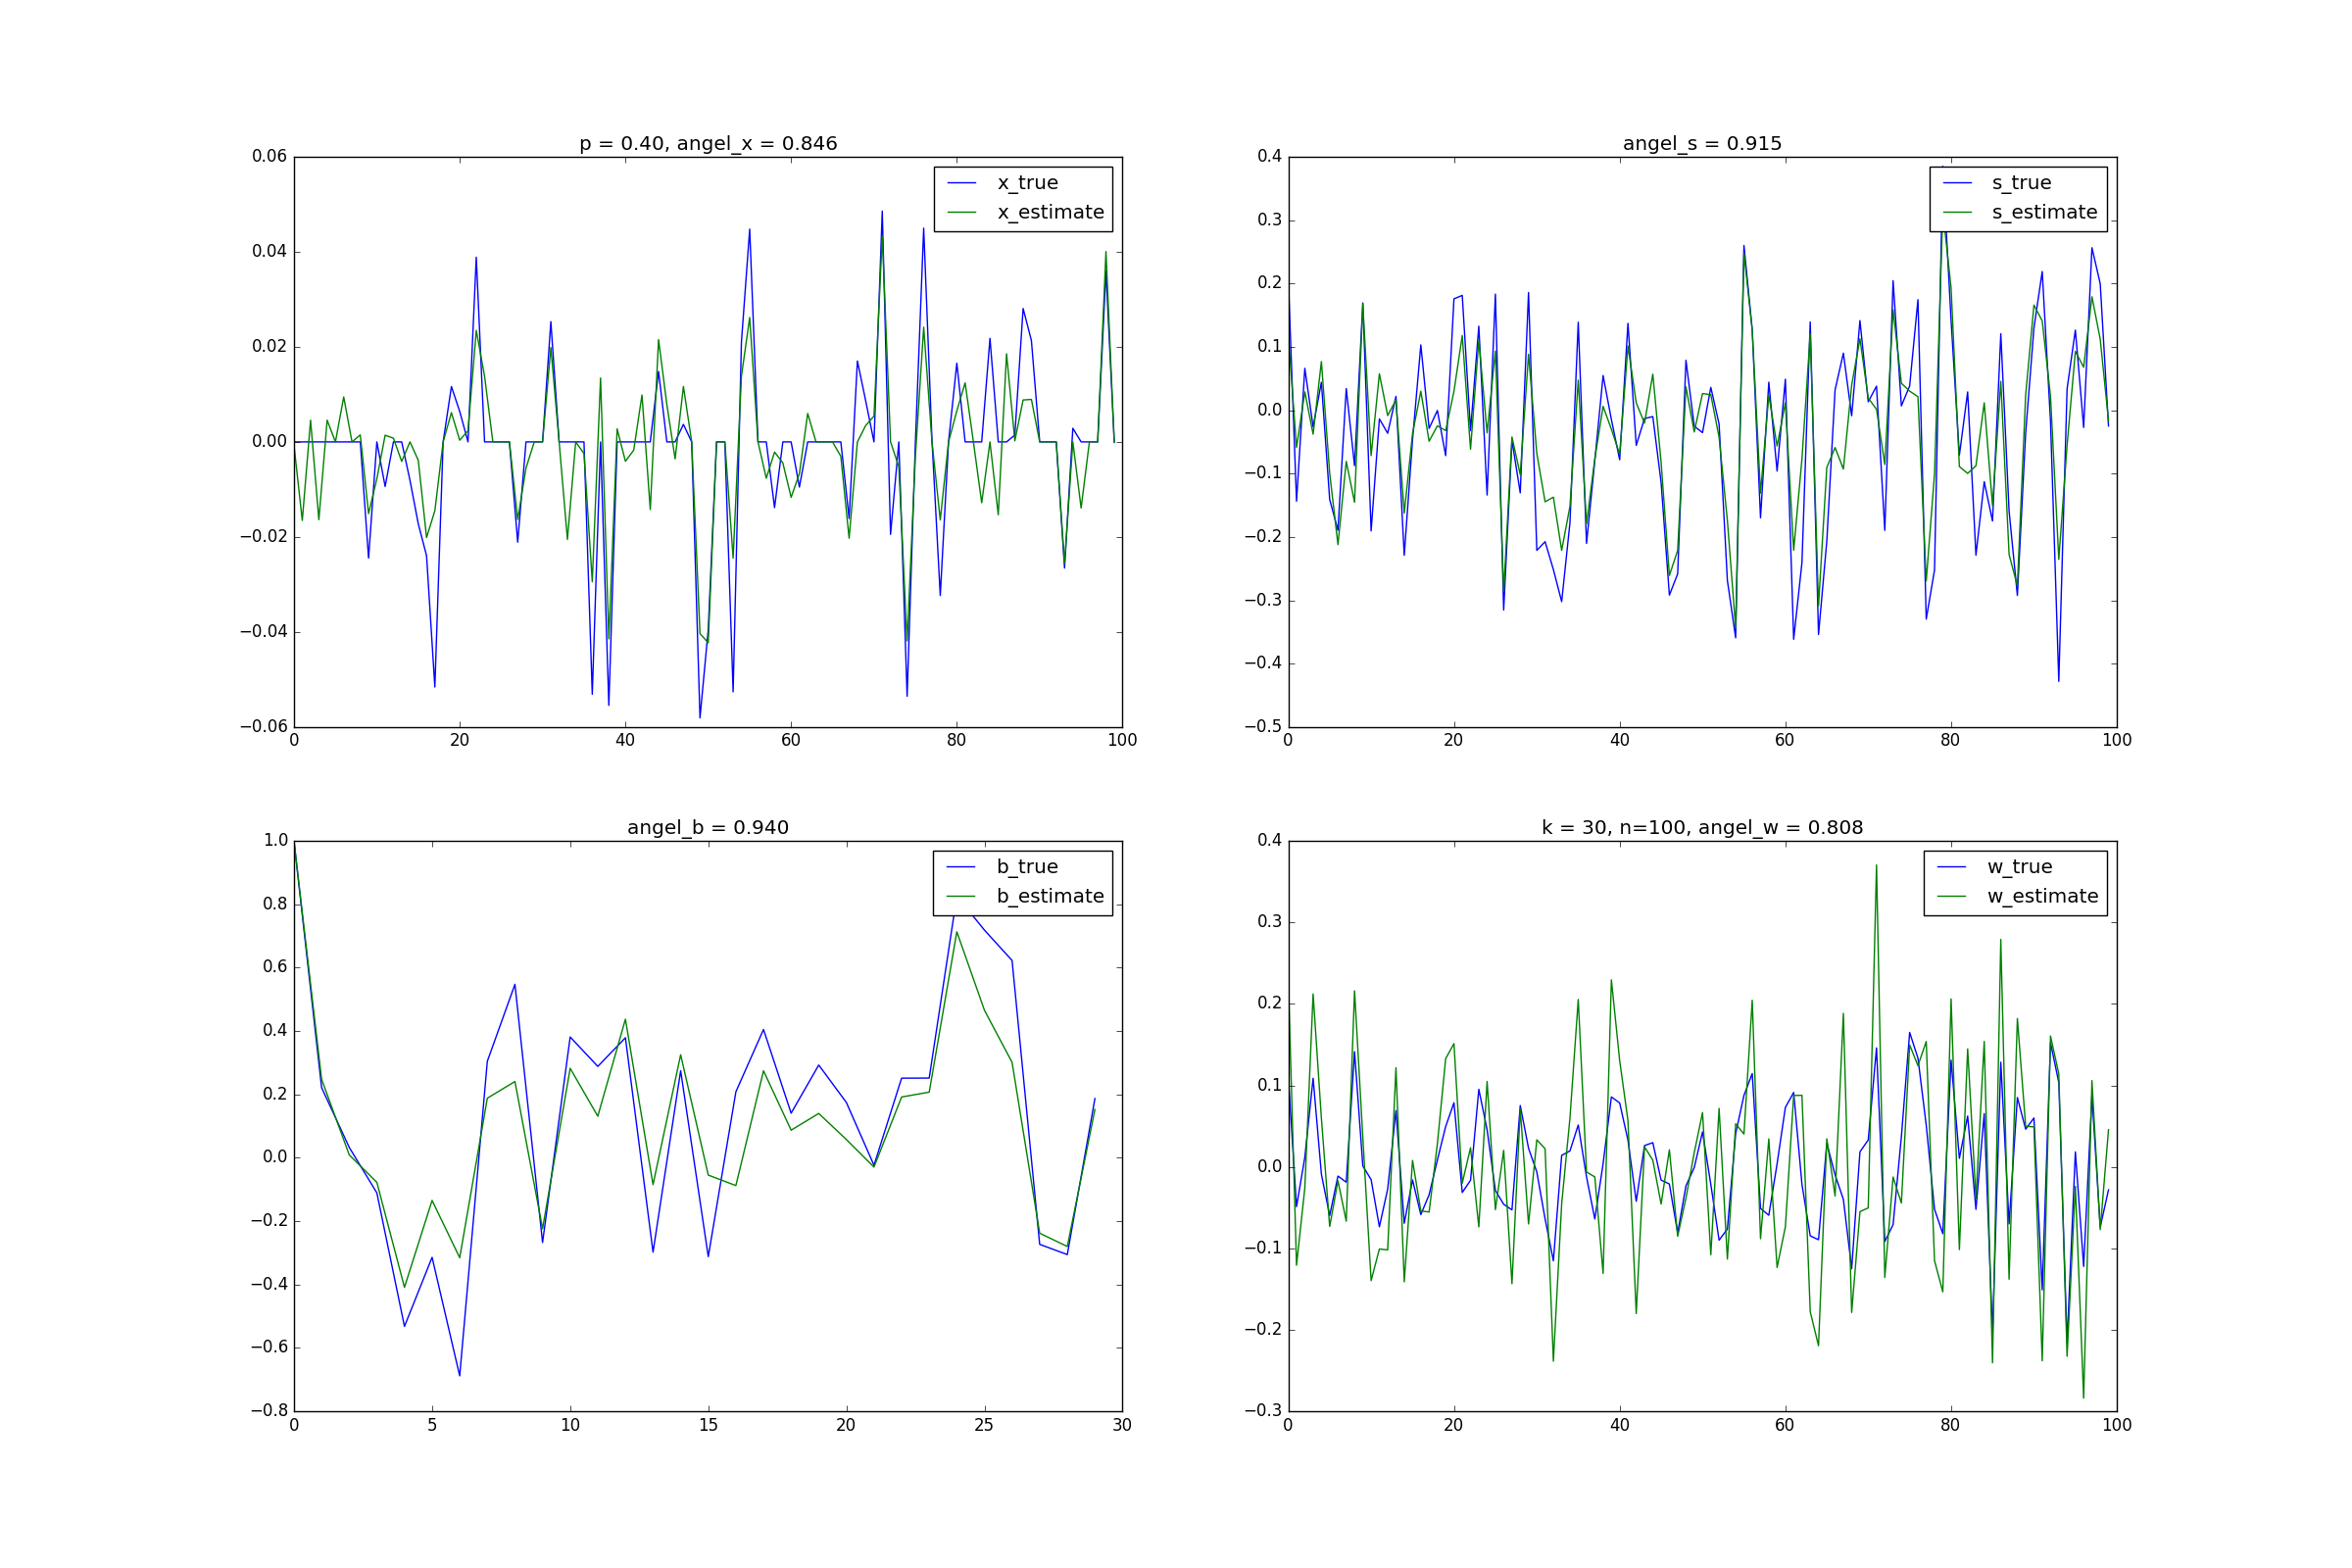
\includegraphics[width=6cm,keepaspectratio]{fig2/bShort_k_lenKnown_xSparse_w_Gaus_AGauss_n100_k30_p0_40_sigma0_00.png}
\caption{Comparison between the ground truth and the estimation for $k=30, p=0.2, 0.4$, the solution is exact at $p=0.2$, the solution is reasonable at $p=0.4$.  }
\end{figure}

\subsubsection{The robustness of the algorithm with incorrect length}
Now we study how robust is the algorithm when we choose the wrong $k$ in the convex problem. We show that when $k'$ is within a certain range of $k$, the solution is still close to the solution with correct length $k'=k$, but when $k'$ is out of that range different solution appears and the solution is off. 

As we saw, when $k=20, p=0.2$ in the generative model, if we choose the length $k'$ of $b$ to be $20$ in the convex problem, the solution is exact, when $k'= 50,$ the solution is still reasonably close, but when $k'= 60,$ the solution is not close.
\begin{figure}
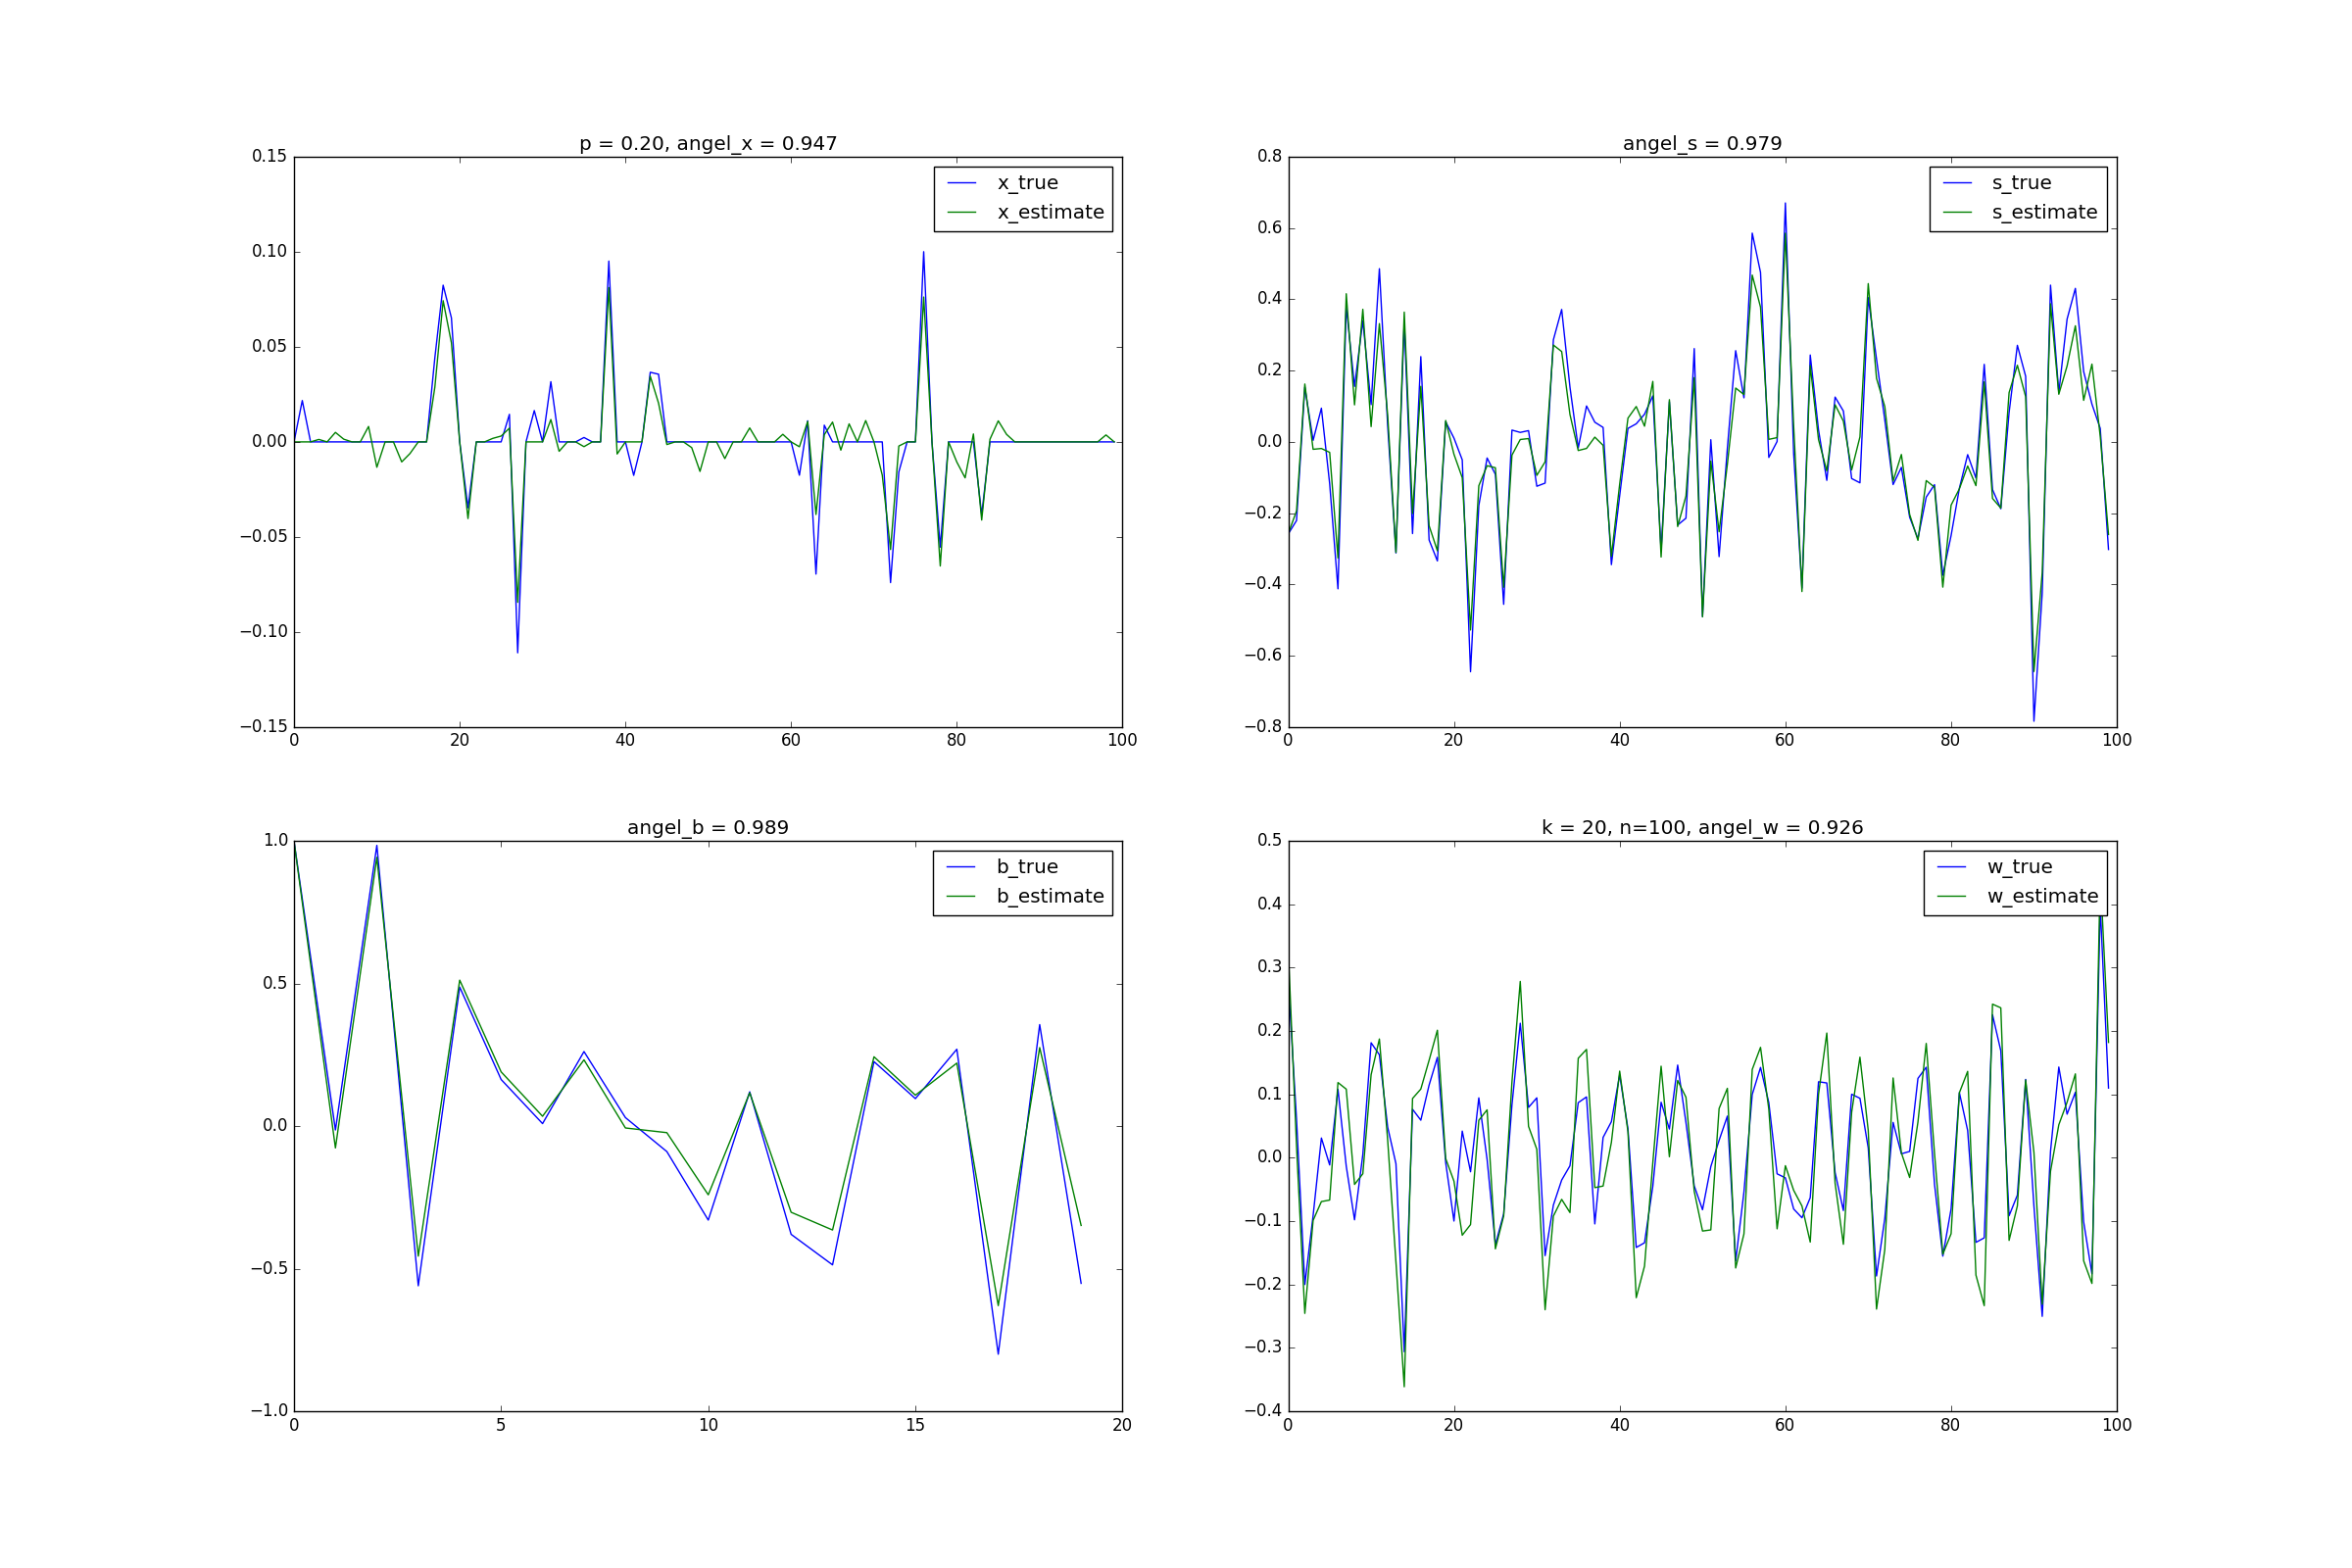
\includegraphics[width=6cm,keepaspectratio]{fig2/03_bShort_wronglen_xSparse_w_Gaus_AGauss_n100_k20_p0_20_sigma0_00.png}
 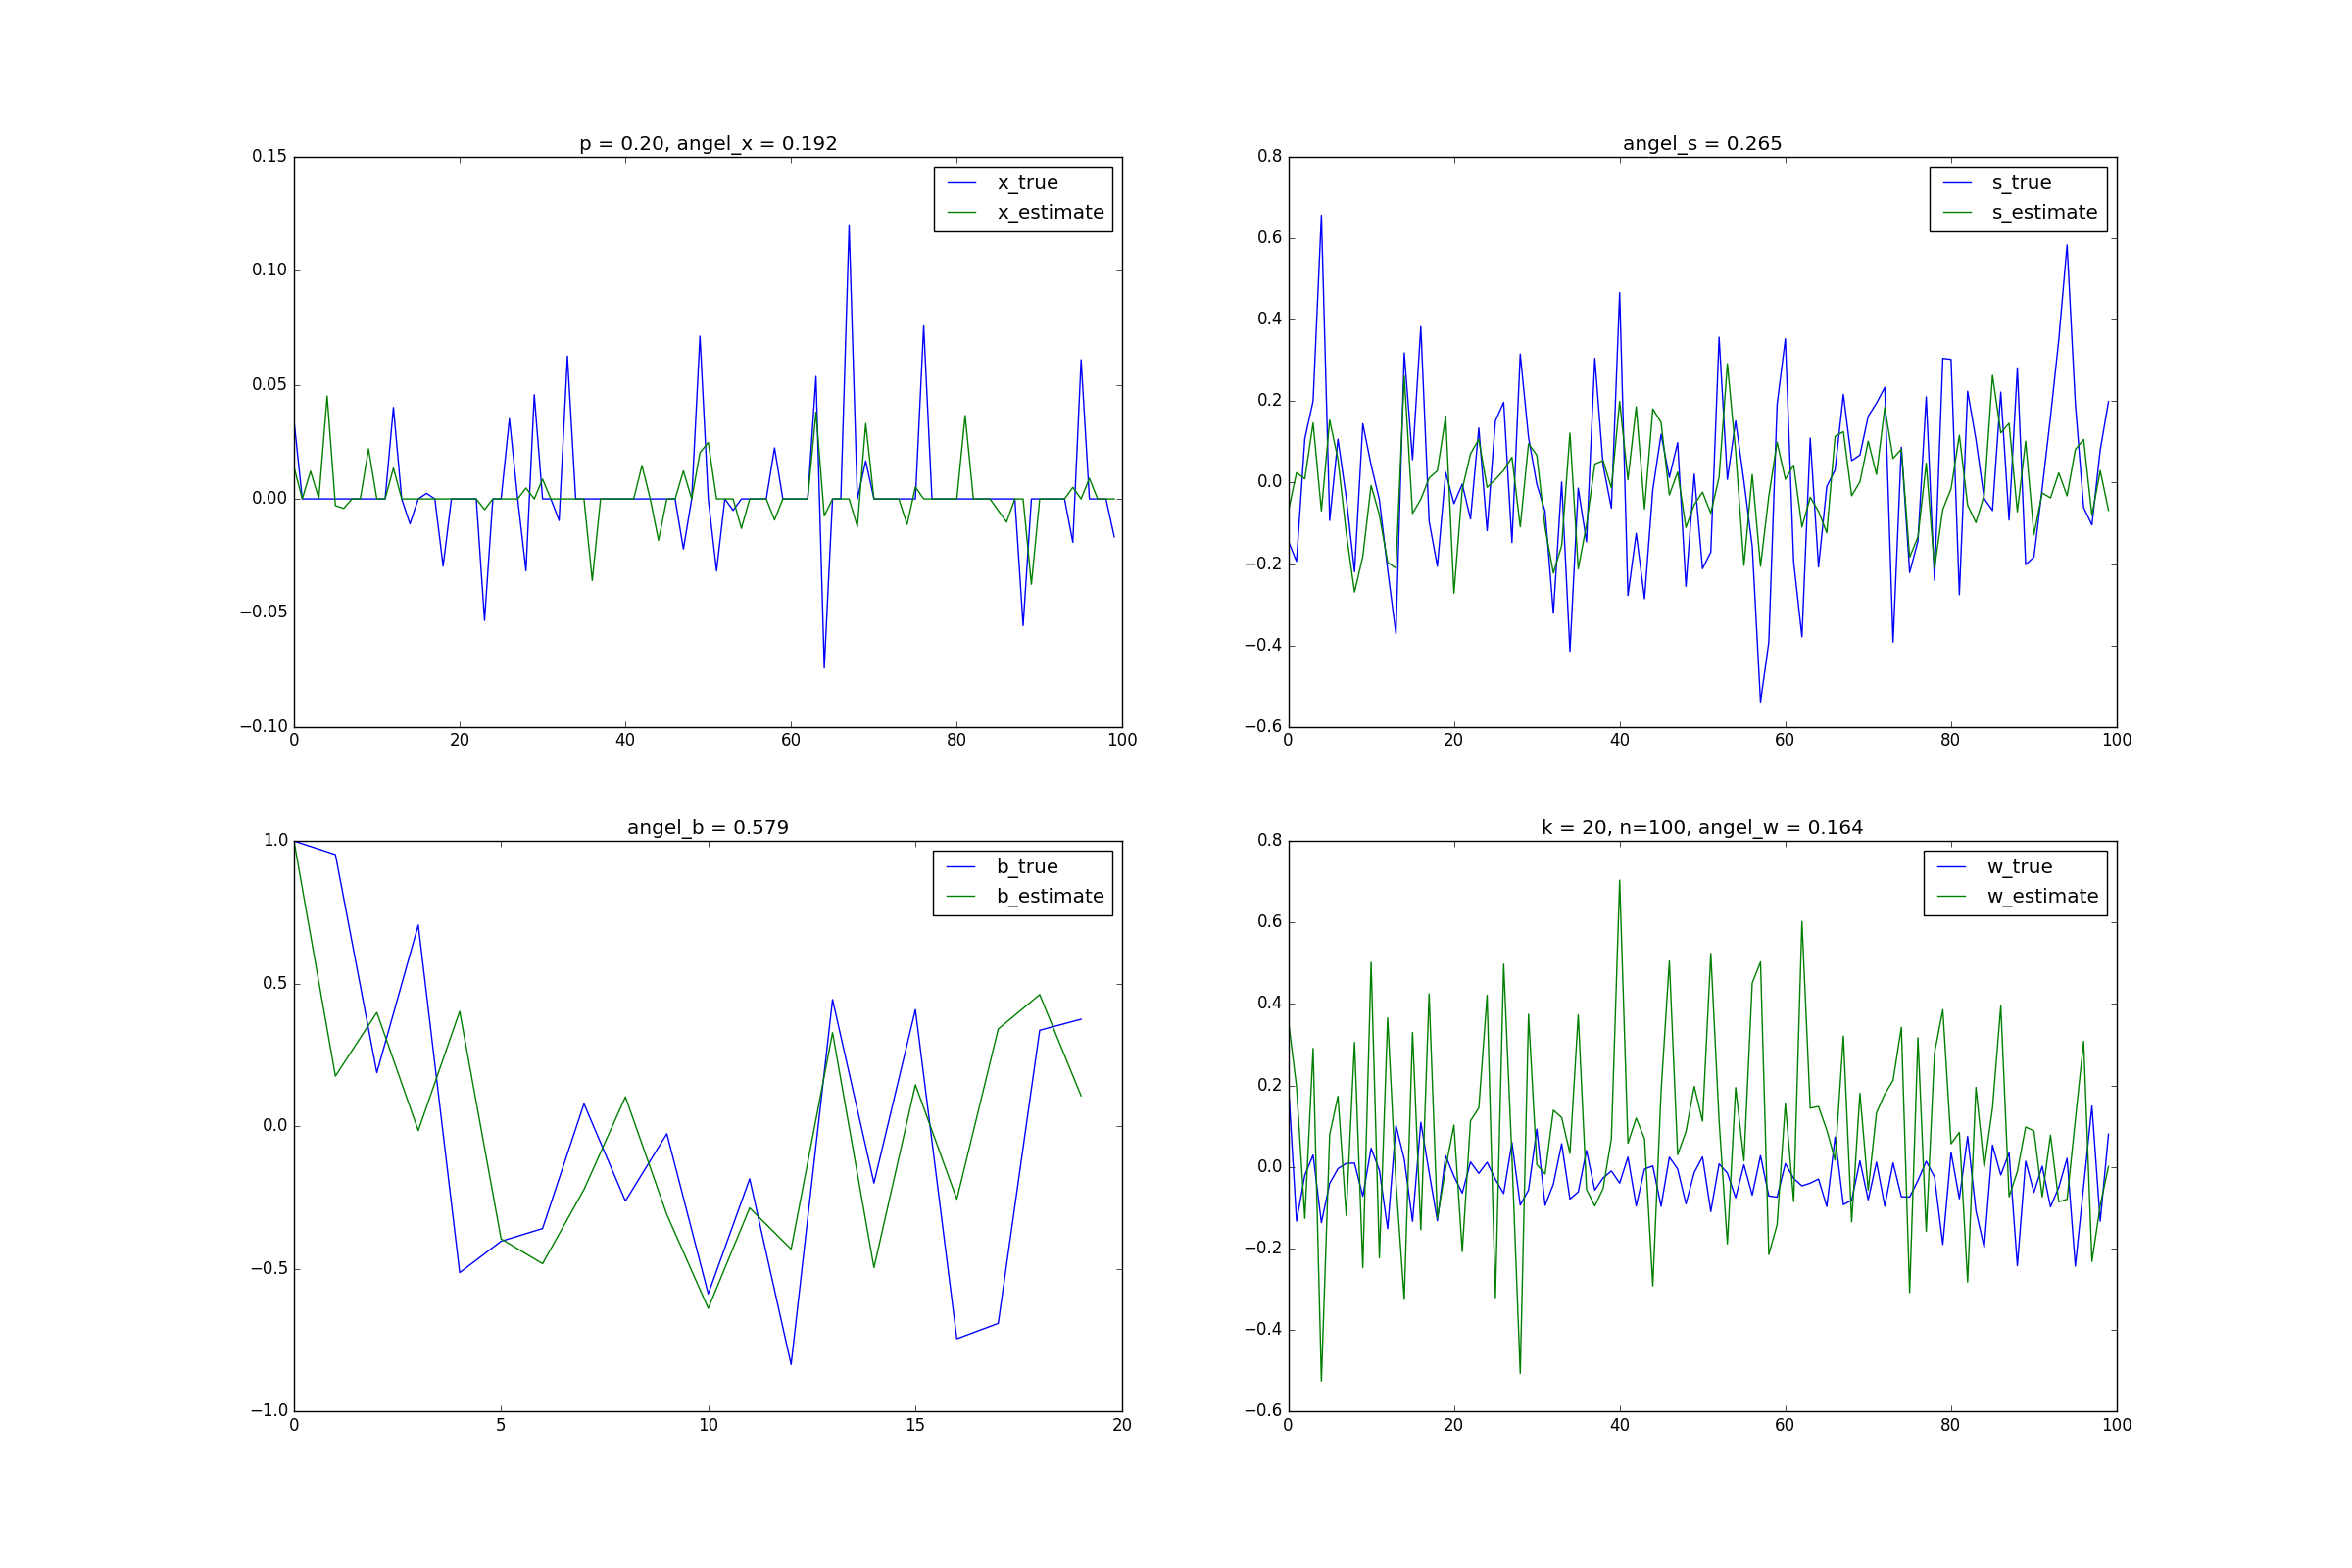
\includegraphics[width=6cm,keepaspectratio]{fig2/03_bShort_k_60_len_xSparse_w_Gaus_AGauss_n100_k20_p0_20_sigma0_00.png}
\caption{Comparison between the ground truth and the estimation for $k=20, p=0.2$, and the first figure is for $k'= 50,$ the second for $k'= 60$, when $k'= 50,$ the solution is still reasonably close, but when $k'= 60,$ the solution is not close. }
\end{figure}

\subsection{Approximating the solution when the kernel is short on different random models}
In the assumption we assume that the inverse kernel is short, but here we show empirically that when the kernel is short but the inverse kernel is not, this approach also gives a good approximation, and  
\subsubsection{Different random models}
Here we first consider the case when $x$ is sparse, namely, the basis $A$ is identity matrix, For the signal $x$,
\begin{itemize}
\item $x\in \mathbb{R}^n$ is I.I.D sampled from product of Bernoulli distribution and standard Gaussian $Ber(p)N(0,1)$.
\item $x\in \mathbb{R}^n$ is I.I.D sampled from the Rademacher distribution, with probability $p/2$ to be $+1$, $p/2$ to be $-1$, $1-p$ to be $0$.
\item $x\in \mathbb{R}^n$ is product of a Gaussian window $f_{gauss}(j) = e^{-(j)^2}$ and I.I.D Bernoulli distribution, $Ber(p)f_{gauss}$.
\item $x\in \mathbb{R}^n$ is product of a cosine window $f_{cos}(j) = cos(j)$ and I.I.D Bernoulli distribution, $Ber(p)f_{cos}$.
\end{itemize}
And $w$ is a kernel of length $k$ generated as following and then padded to length $n$. 
\begin{itemize}
\item $w\in \mathbb{R}^k$ is I.I.D sampled from product from standard Gaussian $N(0,1)$
\item $w\in \mathbb{R}^k$ is sampled from a Gaussian window $e^{-(j)^2}$.
\item $w\in \mathbb{R}^k$ is sampled from a exponential window $w(j) = e^{-|j|}$
\item $w\in \mathbb{R}^k$ is sampled from the cosine window $w(j) = cos(j)$
\end{itemize}

In the experiment, we set $n=100$, and $k= 5, 10, 15, 20, 30$, $p$ change from $0.01$ to $1$, and we measure the angle between the estimated $x$ and $w$ and the corresponding ground truths. As we can see from the experiment the angle is close to $1$ when $k$ and $p$ are both small, and decreasing gradually as $p$ increasing or $k$ increase. It is worth noticing that when $p$ is too small, the convex problem tends to fail.




\begin{figure}
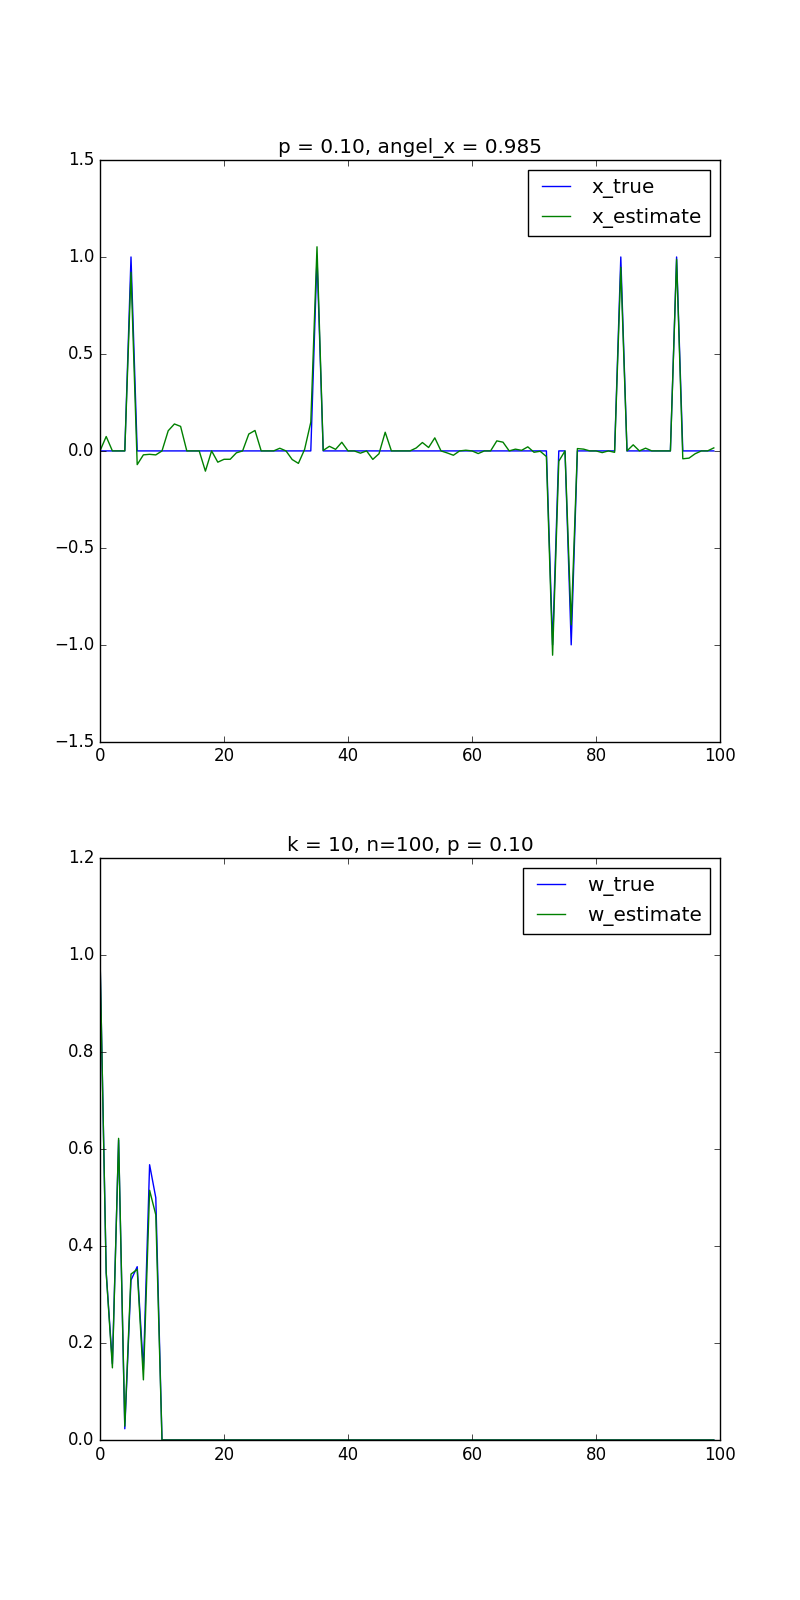
\includegraphics[width=4cm,keepaspectratio]{fig/02_Series_x_Binary_w_Normal_noA_n100_k20_p0_10_sigma0_00.png}
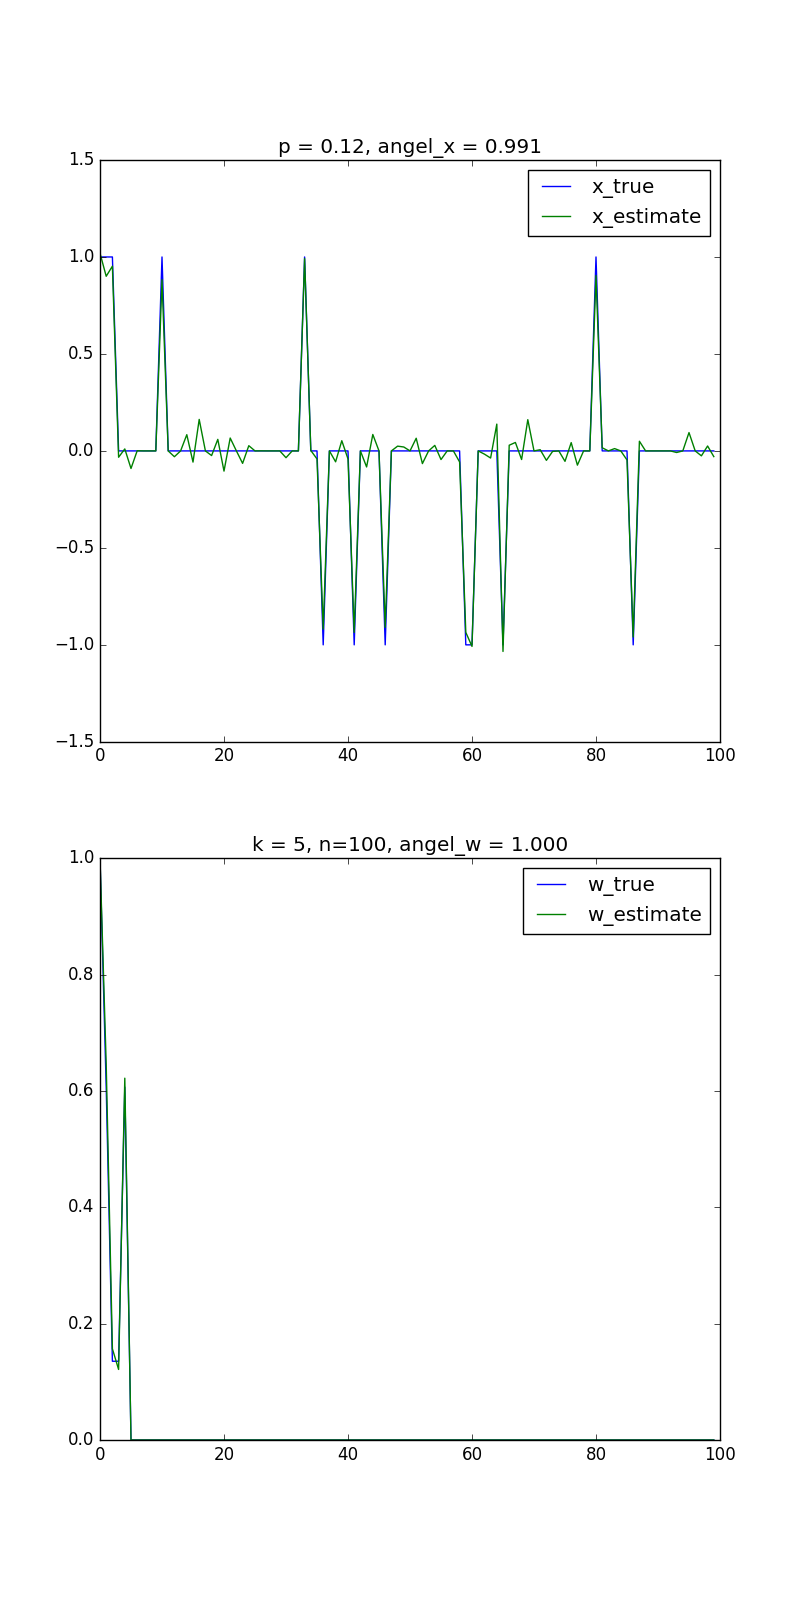
\includegraphics[width=4cm,keepaspectratio]{fig/Collect_Series_x_Binary_w_Gaus_noA_n100_k5_p0_12_sigma0_00.png}
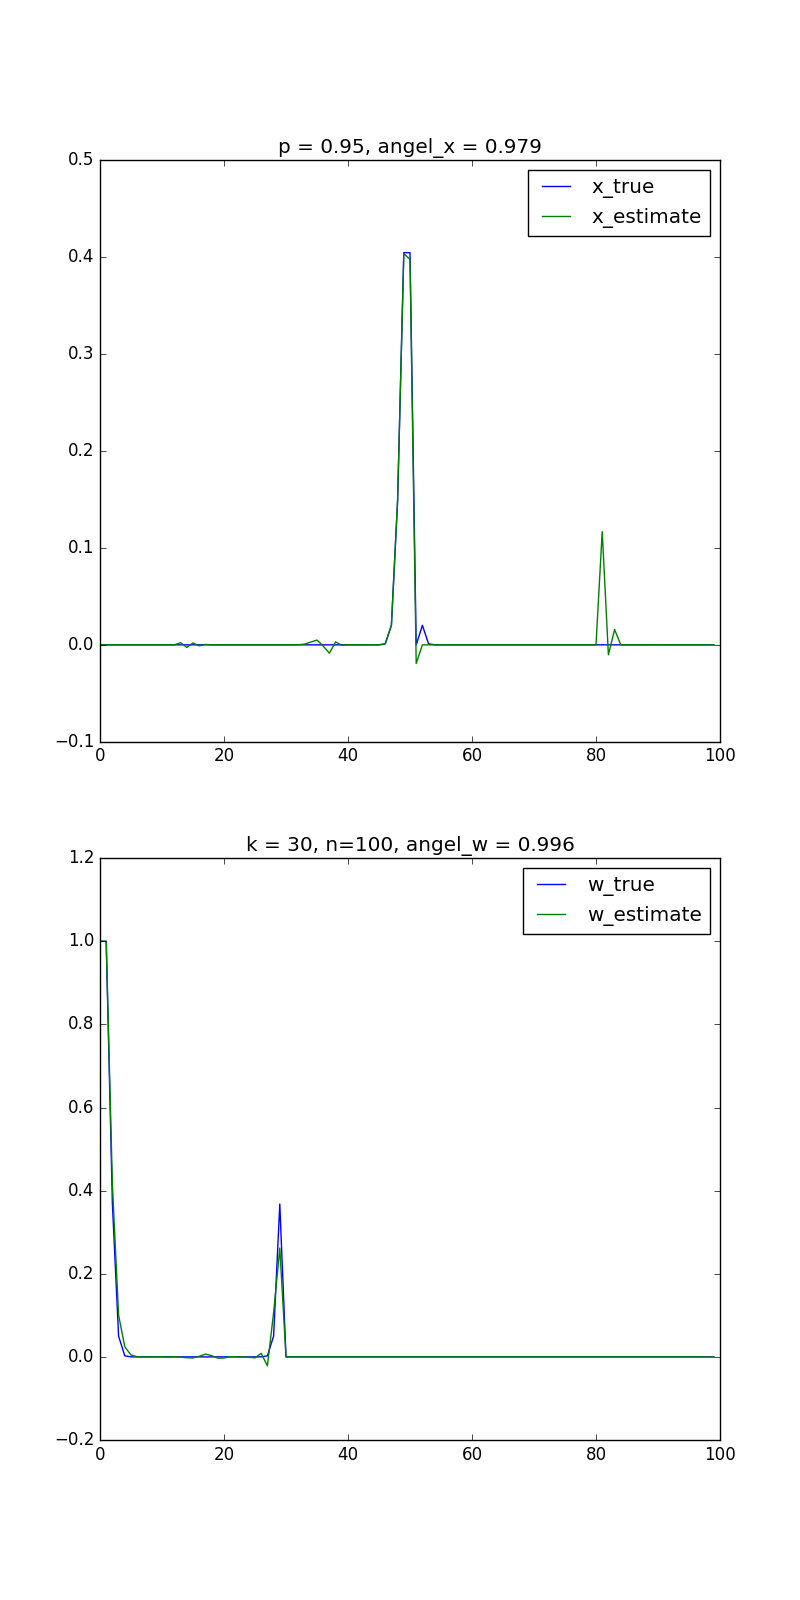
\includegraphics[width=4cm,keepaspectratio]{fig/Collect_Series_x_Gauss_w_Norm_noA_n100_k30_p0_95_sigma0_00.png}
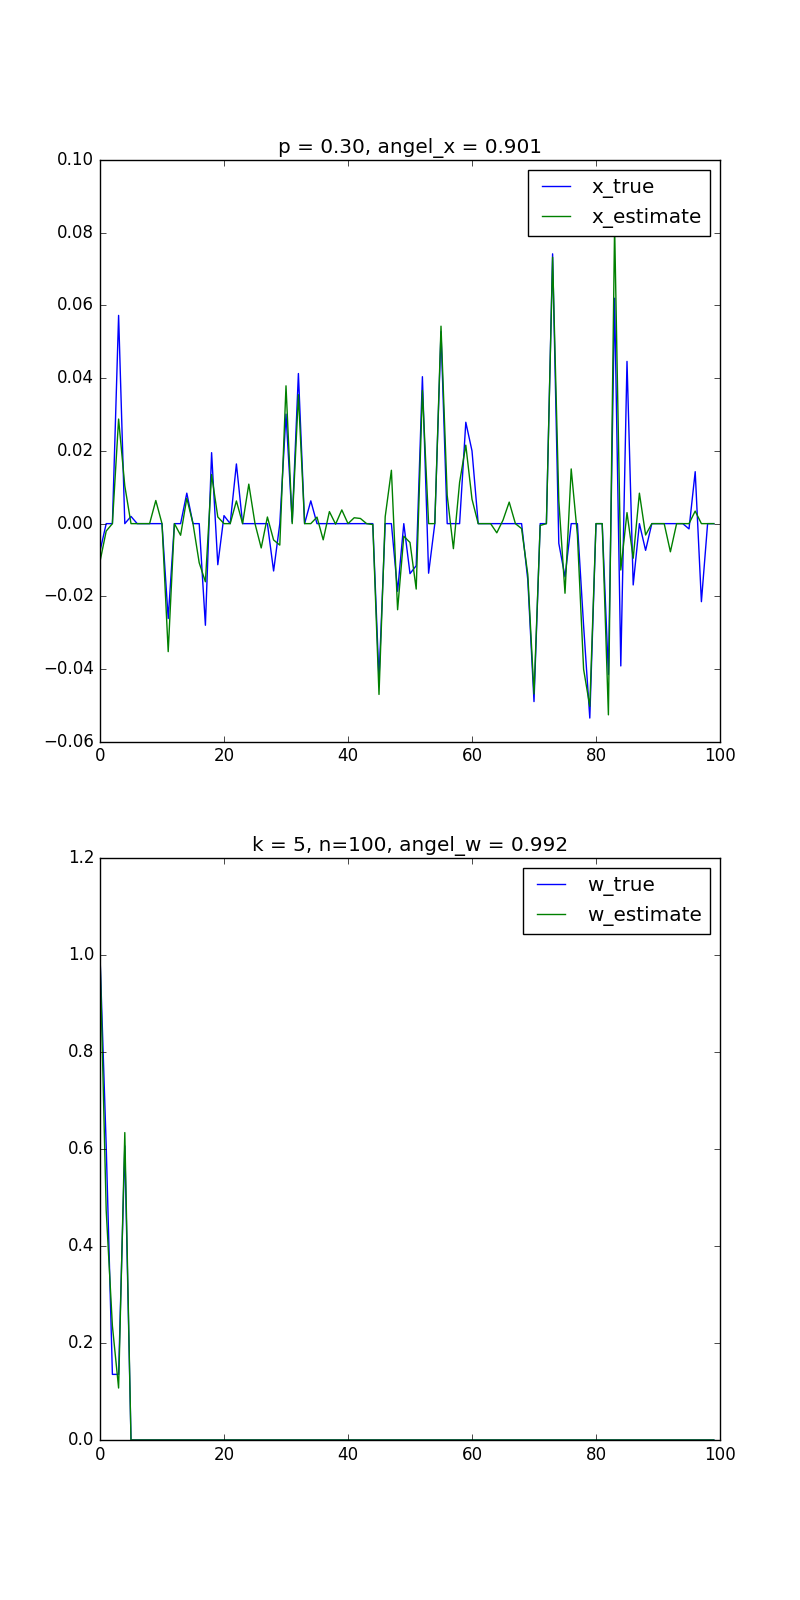
\includegraphics[width=4cm,keepaspectratio]{fig/Collect_Series_x_BernNorm_w_Norm_noA_n100_k5_p0_30_sigma0_00.png}
\caption{Comparison between the ground truth and the estimation. The first is for $x$ binary, I.I.D. sampled from Rademacher distribution, $w$ I.I.D. sampled from standard normal, the second is for $x$ binary, I.I.D. sampled from Rademacher distribution, $w$ sampled from a Gaussian window, the third is for $x$ sampled from a Gaussian window, $w$ I.I.D. sampled from standard normal, the fourth is for $x$ I.I.D. sampled from product of Bernoulli and normal, $w$ I.I.D. sampled from standard normal.}
\end{figure}


\begin{figure}
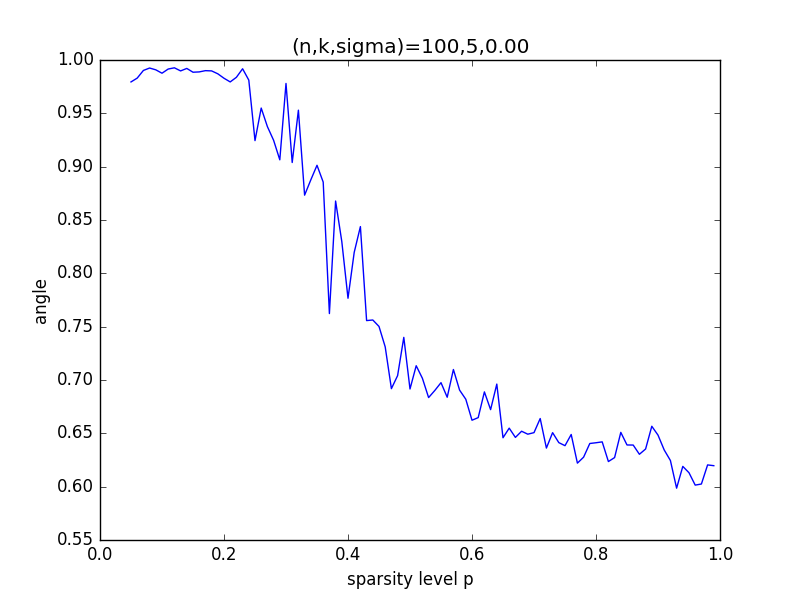
\includegraphics[width=4cm,keepaspectratio]{fig/w_norm_x_binary_n100_k5_p__sigma0_00.png}
 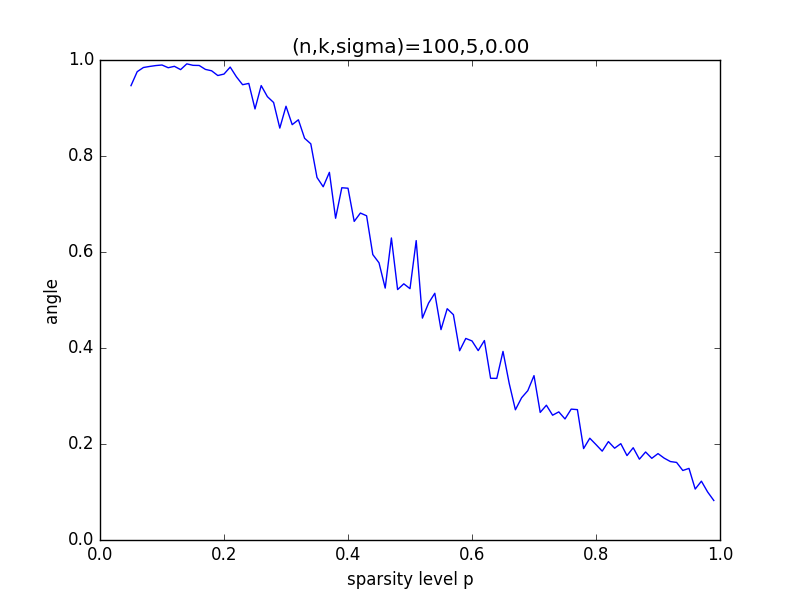
\includegraphics[width=4cm,keepaspectratio]{fig/w_Norm_x_cos_n100_k5_p__sigma0_00.png}
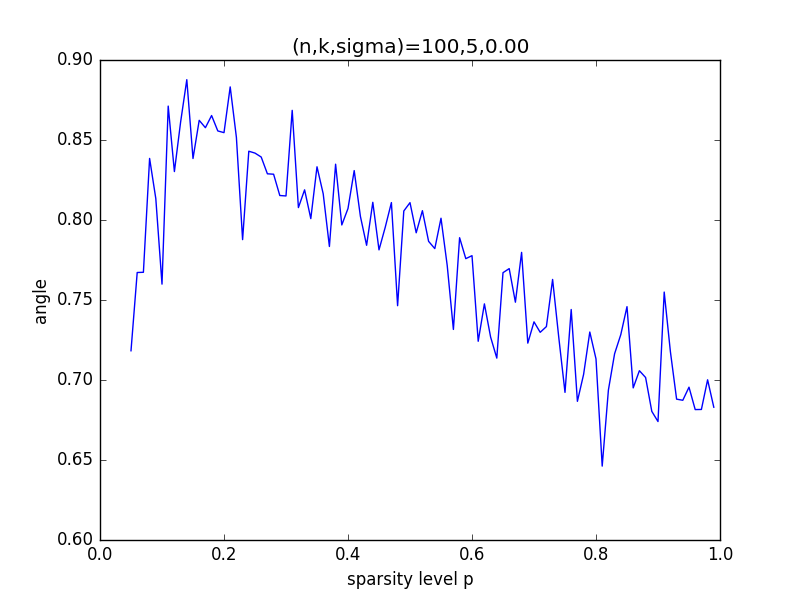
\includegraphics[width=4cm,keepaspectratio]{fig/w_cos_x_BerNorm_n100_k5_p__sigma0_00.png}
\caption{The angle between the estimated $x$ and the ground truth as sparsity level $p$ change. The first is for $x$ binary, I.I.D. sampled from Rademacher distribution, $w$ I.I.D. sampled from standard normal, the second is for $x$ sampled from cosine window, $w$ I.I.D. sampled from standard normal, the third is for $x$ I.I.D. sampled from product of Bernoulli and normal, $w$ sampled from cosine window.}
\end{figure}

\begin{figure}
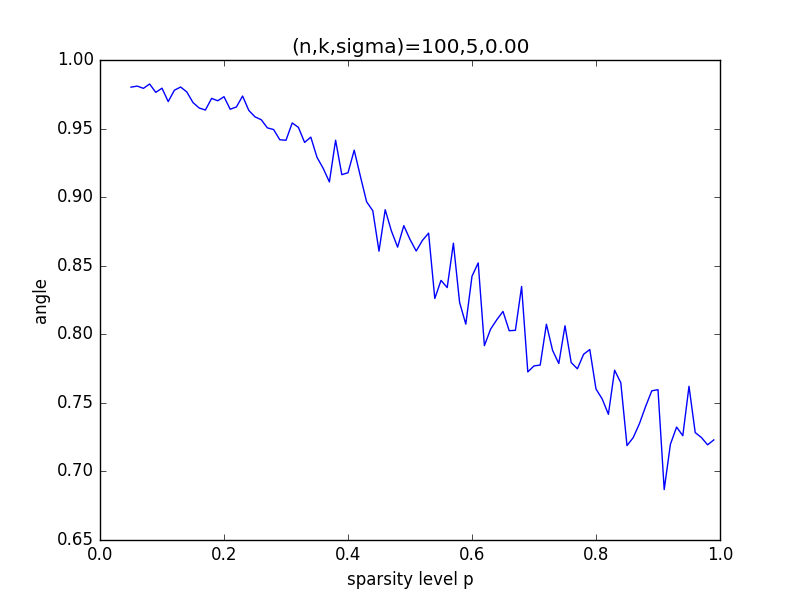
\includegraphics[width=4cm,keepaspectratio]{fig/w_Norm_x_BerNorm_A_Gauss_n100_k5_p__sigma0_00.png}
 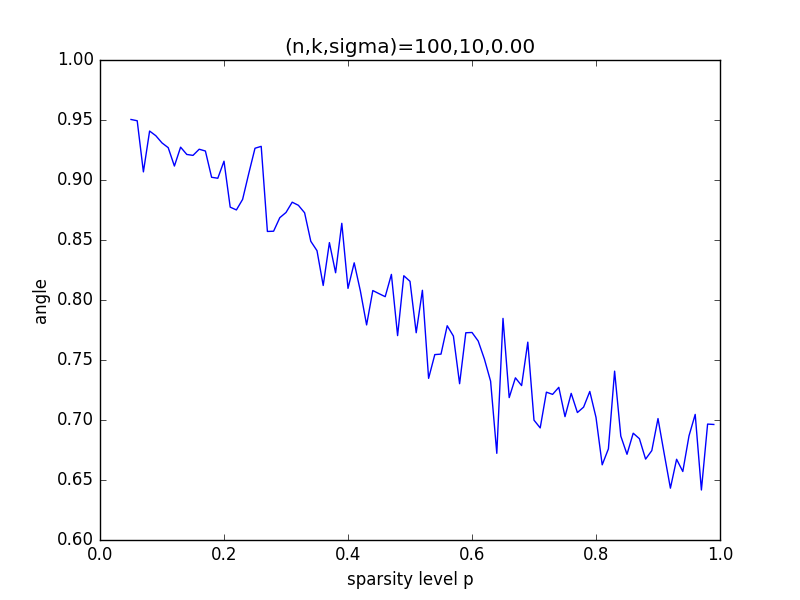
\includegraphics[width=4cm,keepaspectratio]{fig/w_Norm_x_BerNorm_A_Gauss_n100_k10_p__sigma0_00.png}
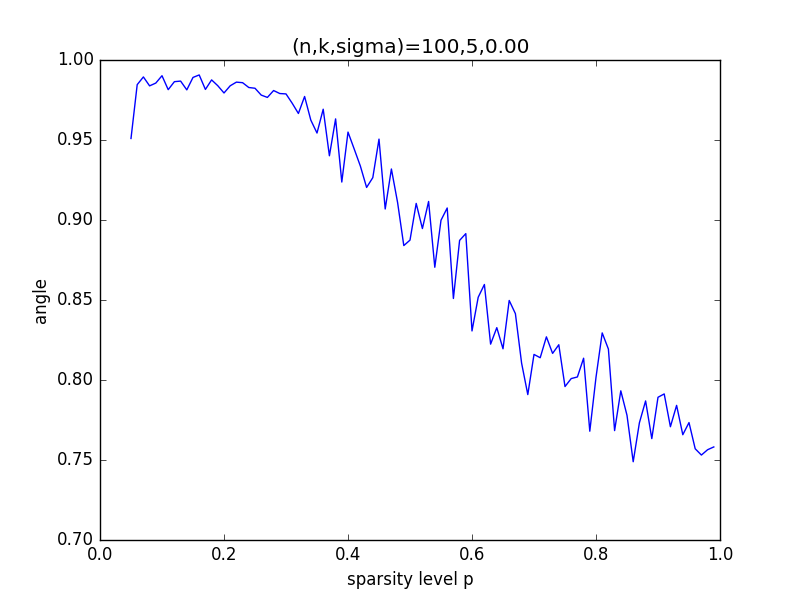
\includegraphics[width=4cm,keepaspectratio]{fig/w_Norm_x_BerNorm_A_none_n100_k5_p__sigma0_00.png}
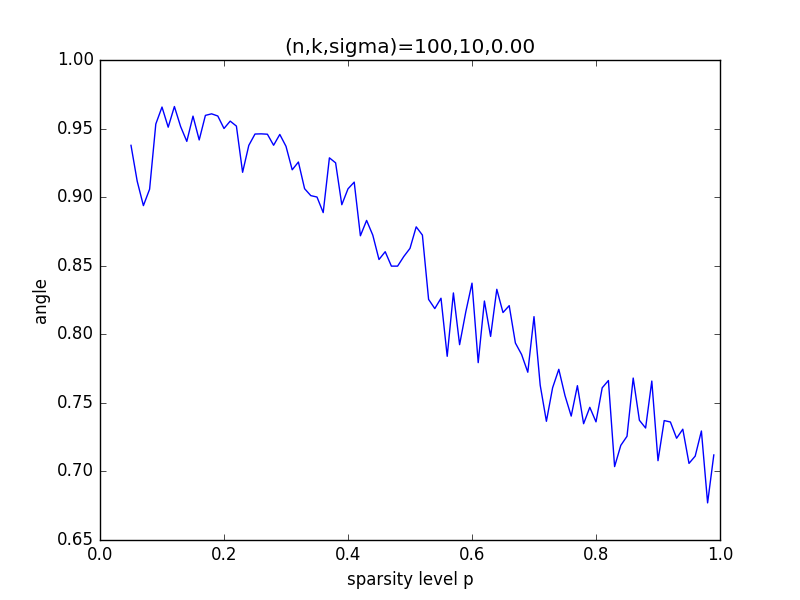
\includegraphics[width=4cm,keepaspectratio]{fig/w_Norm_x_BerNorm_A_none_n100_k10_p__sigma0_00.png}
\caption{The angle between the estimated $x$ and the ground truth for $x$ I.I.D. sampled from product of Bernoulli and normal, $w$ I.I.D. sampled from standard normal. The first and second are for $A=I$ with $k=5,10$, the third and fourth are for $A$ $n\times n$ Gaussian random matrix, with $k=5,10$.   }
\end{figure}


%\indent {\bf Acknowledgement.} 

%\newpage
%\tableofcontents 
%\newpage 






{\small
\bibliographystyle{amsalpha}
\bibliography{ncvx,spm}
}

\end{document}


